 \documentclass[notitlepage]{article}
\usepackage[left=1in, right=1in, top=1in, bottom=1in]{geometry}
%% Language and font encodings
\usepackage[english]{babel}
\usepackage{morewrites}




%\selectlanguage{spanish}
\usepackage[utf8x]{inputenc}
\usepackage[nolist]{acronym}
\usepackage{etoolbox}
\usepackage{graphicx}
\usepackage{titling}
\usepackage[threshold=1]{csquotes}
\usepackage{setspace}
\usepackage{soul}
\usepackage{color}
\usepackage[usenames,dvipsnames,table]{xcolor}


\usepackage{cite}


\usepackage{enumitem}
\newenvironment{packed_enum}{
\begin{enumerate}
  \setlength{\itemsep}{-1pt}
  \setlength{\parskip}{0pt}
  \setlength{\parsep}{0pt}
}{\end{enumerate}}
\usepackage{multicol}
\usepackage{multirow}
\newcolumntype{L}[1]{>{\raggedright\let\newline\\\arraybackslash\hspace{0pt}}p{#1}}
\newcolumntype{C}[1]{>{\centering\let\newline\\\arraybackslash\hspace{0pt}}m{#1}}
\newcolumntype{R}[1]{>{\raggedleft\let\newline\\\arraybackslash\hspace{0pt}}m{#1}}
\makeatletter
\def\hlinewd#1{%
\noalign{\ifnum0=`}\fi\hrule \@height #1 %
\futurelet\reserved@a\@xhline} 
\makeatother

%%%%%%%%%%%%%%%%%%%%%%%%%%%%%%%%%%%%%%%
%%SETTING BIBLIOGRAPHY FORMAT
%%%%%%%%%%%%%%%%%%%%%%%%%%%%%%%%%%%%%%%
%\usepackage{multibbl}
%\addto{\captionsenglish}{\renewcommand{\bibname}{}}
%\renewcommand{\bibname}{}
%\patchcmd{\thebibliography}{\chapter*}{\subsection*}{}{}
%\let\oldbibliography\thebibliography
%\renewcommand{\thebibliography}[1]{%
%  \oldbibliography{#1}%
%  \setlength{\itemsep}{0pt}%
%}


%%%%%%%%%%%%%%%%%%%%%%%%%%%%%%%%%%%%%%
%CUSTOM COMMANDS
%%%%%%%%%%%%%%%%%%%%%%%%%%%%%%%%%%%%%%

%\renewcommand\thesection{\arabic{section}}


%%%%%%%%%%%%%%%%%%%%%%%%%%%%%%%%%%%%%%
%EXAMINATION COMMITTEE NAMES AND CREDENTIALS
%%%%%%%%%%%%%%%%%%%%%%%%%%%%%%%%%%%%%%
\newcommand{\compr}{Danielle Wood}
\newcommand{\comte}{David Lagomasino}
\newcommand{\comco}{Sarah Williams}

\newcommand{\comprcredentials}{\newline\indent Assistant Professor of Media Arts and Sciences \newline\indent Program in Media Arts and Sciences \newline\indent Assistant Professor (Joint) of Aeronautics and Astronautics \newline\indent Department of Aeronautics and Astronautics \newline\indent Massachusetts Institute of Technology}

\newcommand{\comtecredentials}{\newline\indent Assistant Professor of Coastal Studies \newline\indent Department of Coastal Studies \newline\indent East Carolina University}

\newcommand{\comcocredentials}{\newline\indent Associate Professor of Technology and Urban Planning \newline\indent  Director of the Norman B. Leventhal Center for Advanced Urbanism \newline\indent Urban Science and Computer Science Program \newline\indent Department of Urban Studies and Planning \newline\indent Massachusetts Institute of Technology}

%%%%%%%%%%%%%%%%%%%%%%%%%%%%%%%%%%%%%%
%AREA NAMES
%%%%%%%%%%%%%%%%%%%%%%%%%%%%%%%%%%%%%%
\newcommand{\Apr}{Socio-environmental-technical Systems Design, Modeling, and Decision-Making}
\newcommand{\Ate}{Remote Observation of Natural and Social Phenomena}
\newcommand{\Aco}{Development, Data, and Justice in Socio-environmental-technical Systems}

%\usepackage{titlesec}
%\titleformat{\section}{\normalfont\Large\bfseries}{}{0pt}{}

%%%%%%%%%%%%%%%%%%%%%%%%%%%%%%%%%%%%%%
%ACRONYMS
%%%%%%%%%%%%%%%%%%%%%%%%%%%%%%%%%%%%%%
\begin{acronym}[VALUABLES]
	\acro{eo}[EO]{earth observation}
	\acro{nasa}[NASA]{National Aeronautics and Space Administration}
%	\acro{usaid}[USAID]{United States Agency for International Development}
%	\acro{servir}[SERVIR]{Sistema Regional De Visualizaci\'{o}n Y Monitoreo De Mesoam\'{e}rica}
	\acro{eos}[EOS]{Earth Observation System}
	%\acro{geo}[GEO]{Group of Earth Observations}
	\acro{osse}[OSSE]{Observing System Simulation Experiment}
	%\acro{un}[UN]{United Nations}
	%\acro{mdg}[MDG]{Millennium Development Goal}
	\acro{sdg}[SDG]{Sustainable Development Goal}
	\acro{fews}[FEWS NET]{Famine Early Warning Systems Network}
	%\acro{fema}[FEMA]{Federal Emergency Management Agency}
	%\acro{jpl}[JPL]{Jet Propulsion Laboratory}
	%\acro{dod}[DoD]{Department of Defense}
	\acro{osse}[OSSE]{Observing System Simulation Experiment}
	\acro{ngo}[NGO]{non-governmental organization}
	\acro{noaa}[NOAA]{National Oceanic and Atmospheric Administration}
	%\acro{firms}[FIRMS]{Fire Information for Resource Management System}
	\acro{ceos}[CEOS]{Committee on Earth Observation Satellites}
	\acro{gis}[GIS]{geospatial information system}
	%\acro{esa}[ESA]{European Space Agency}
	%\acro{cbers}[CBERS]{China-Brazil Earth Resources Satellite Program}
	%\acro{jaxa}[JAXA]{Japan Aerospace Exploration Agency}
	%\acro{eoc}[EOC]{Earth Observation Center}
	%\acro{usgs}[USGS]{US Geological Survey}
	%\acro{ipcc}[IPCC]{Intergovernmental Panel on Climate Change}
	%\acro{cad}[CAD]{computer-aided design}
	%\acro{arl}[ARL]{Application Readiness Level}
	%\acro{trl}[TRL]{Technology Readiness Level}
	%\acro{mbse}[MBSE]{model-based systems engineering}
	%\acro{siurb}[SIURB]{Sistema Municipal de Informa\c{c}\~{o}es Urbanas}
	\acro{dss}[DSS]{decision support system}
	\acro{evdt}[EVDT]{Environment, Vulnerability, Decision-Making, Technology}
	\acro{aiaa}[AIAA]{American Institute of Aeronautics and Astronautics}
	\acro{cas}[CAS]{complex adaptive system}
	\acro{cbers}[CBERS]{China-Brazil Earth Resources Satellite Program}
	\acro{ceos}[CEOS]{Committee on Earth Observation Satellites}
	\acro{cpr}[CPR]{common-pool resources}
		\acro{dem}[DEM]{Digital Elevation Model}
	\acro{dsm}[DSM]{Digital Surface Model}
	\acro{dss}[DSS]{Decision Support System}
	\acro{dtm}[DTM]{Digital Terrain Model}
	\acro{eo}[EO]{earth observation}
	\acro{eoc}[EOC]{Earth Observation Center}
	\acro{eos}[EOS]{earth observation system}
	\acro{epa}[EPA]{Environmental Protection Agency}
	\acro{esa}[ESA]{European Space Agency}
	\acro{evdt}[EVDT]{Environment, Vulerability, Decision-Making, Technology}
	\acro{fema}[FEMA]{Federal Emergency Management Agency}
	\acro{geo}[GEO]{Group of Earth Observations}
	\acro{fews}[FEWS NET]{Famine Early Warning Systems Network}
	\acro{gis}[GIS]{geographic information system}
	\acro{gisc}[GISc]{geographic information science}
	\acro{gpm}[GPM]{Global Precipitation Measurement}
	\acro{grace}[GRACE]{Gravity Recovery and Climate Experiment}
	\acro{icesat2}[ICESat-2]{Ice, Cloud, and land Elevation Satellite 2}
	\acro{ilute}[ILUTE]{Integrated Land Use, Transportation, Environment}
	\acro{jaxa}[JAXA]{Japan Aerospace Exploration Agency}
	\acro{leed}[LEED]{Leadership in Energy and Environmental Design}
	\acro{lidar}[LIDAR]{light detection and ranging}
	\acro{lunr}[LUNR]{Land Use and Natural Resources Inventory}
	\acro{mdg}[MDG]{Millenium Development Goal}
	\acro{modis}[MODIS]{Moderate Resolution Imaging Spectroradiometer}
	\acro{nasa}[NASA]{National Aeronautics and Space Administration}
	\acro{noaa}[NOAA]{National Oceanic and Atmospheric Administration}
	\acro{ngo}[NGO]{non-governmental organization}
	\acro{ostp}[OSTP]{Office of Science and Technology Policy}
	\acro{ota}[OTA]{Office of Technology Assessment}
	\acro{pgis}[PGIS]{participatory geographic information system}
	\acro{ppgis}[PPGIS]{public participation geographic information system}
	\acro{ppbs}[PPBS]{Planning-Programming-Budgeting System}
	\acro{pss}[PSS]{Planning Support System}
	\acro{sdg}[SDG]{Sustainable Development Goal}
	\acro{servir}[SERVIR]{Sistema Regional De Visualizaci\'{o}n Y Monitoreo De Mesoam\'{e}rica}
	\acro{swot}[SWOT]{Surface Water Ocean Topography}
	\acro{un}[UN]{United Nations}
	\acro{usaid}[USAID]{United States Agency for International Development}
	\acro{usgs}[USGS]{United States Geological Survey}
	\acro{viirs}[VIIRS]{Visible Infrared Imaging Radiometer Suite}
	\acro{iso}[ISO]{international standards organization}
	\acro{iec}[IEC]{International Electrotechnical Commission}
	\acro{ieee}[IEEE]{Institute of Electrical and Electronics Engineers}
	\acro{sebok}[SEBoK]{Systems Engineering Body of Knowledge}
	\acro{incose}[INCOSE]{International Council on Systems Engineering}
	\acro{sets}[SETS]{Socio-environmental-technical System}
	\acro{sts}[STS]{Sociotechnical system}
	\acro{ses}[SES]{Socio-environmental system}
	\acro{osse}[OSSE]{Observing System Simulation Experiment}
	\acro{ipp}[IPP]{the Pereira Passos Municipal Institute of Urbanism}
	\acro{ipm}[IPM]{Multidimensional Poverty Index}
	\acro{ufrj}[UFRJ]{Federal University of Rio de Janeiro}
	\acro{gee}[GEE]{Google Earth Engine}
	\acro{gmw}[GMW]{Global Mangrove Watch}
	\acro{daac}[DAAC]{Distributed Active Archive Centers}
	\acro{ceos}[CEOS]{the Committee on Earth Observation Satellites}
	\acro{eo4sdg}[EO4SDG]{Earth Observation for the Sustainable Development Goals}
	\acro{ibge}[IBGE]{Brazilian Institute of Geography and Statistics}
	\acro{mit}[MIT]{Massachusetts Institute of Technology}
\end{acronym}

%%%%%%%%%%%%%%%%%%%%%%%%%%%%%%%%%%%%%%
%TITLE PAGE & TABLE OF CONTENTS
%%%%%%%%%%%%%%%%%%%%%%%%%%%%%%%%%%%%%%
\begin{document}
\pretitle{\begin{center}\Huge\bfseries}
\posttitle{\par\end{center}\vskip 0.5em}
\preauthor{\begin{center}\Large\ttfamily}
\postauthor{\end{center}}
\predate{\par\large\centering}
\postdate{\par}

\title{Using Integrated Earth Observation-Informed Modeling to Inform Sustainable Development Decision-Making \\  
\large Ph.D. Thesis Proposal} 
\author{%
Jack Reid\\ 
Space Enabled Research Group\\
MIT Media Lab\\
jackreid@mit.edu}

\maketitle

\section*{Supervising Committee}


\vspace{\baselineskip}

\textbf{\compr} \comprcredentials 
 
\vspace{\baselineskip}

\textbf{\comte} \comtecredentials

\vspace{\baselineskip}

\textbf{\comco} \comcocredentials

\thispagestyle{plain}
\pagestyle{plain}

\clearpage
%\tableofcontents

%%%%%%%%%%%%%%%%%%%%%%%%%%%%%%%%%%%%%%
\section*{Abstract}
%%%%%%%%%%%%%%%%%%%%%%%%%%%%%%%%%%%%%%

%[A short overview of the key goals, questions, and expected contributions.]

Over the past two decades satellite-based remote observation has blossomed. We have seen a rapid increase in the number of \acp{eos} in orbit, significant improvements in their capabilities, and much greater availability of the data that they produce. This trend has occurred as part of a greater trend of increasing data availability, computational power, and modeling ability. Unfortunately, up until now, this \ac{eo} data has been largely used only by governments and academics for scientific purposes, typically to understand and predict environmental phenomena. Large corporations and \acp{ngo} have recently been conducting their own analyses, but these have required significant expertise and resources, and the results have sadly been mostly unavailable to the broader public. 

There is a real need for (a) making remote observation data not just available but accessible to a broader audience by developing data products that are relevant to everyday individuals, particularly those involved in local, rather than national or global decision-making; (b) linking the \ac{eo}-supported environmental modeling with the societal impact of a changing environment; and (c) putting policy and sensor design decision-making in the hands of a broader population. 

This work aims to demonstrate the viability of a particular methodology for achieving (a) and (b), while laying the groundwork for a more detailed consideration of (c). To that end, this work centers on exploring the efficacy and difficulties of \textbf{\textit{collaboratively developing}} a \textbf{\textit{systems-architecture-informed}}, multidisciplinary \textbf{\textit{\ac{gis} \ac{dss}}} for \textbf{\textit{sustainable development}} applications that makes significant use of \textbf{\textit{remote observation data}}. 

This is done through the development and evaluation of \acp{dss} for two primary applications: (1) mangrove forest management and conservation in the state of Rio de Janeiro, Brazil; and (2) coronavirus response in six metropolitan areas across Angola, Brazil, Chile, Indonesia, Mexico, and the United States. In both cases, the methodology involves the application the system architecture framework, an approach that has been previously adapted from the aerospace engineering discipline by Prof. Wood for use in sociotechnical systems. This includes using stakeholder mapping and network analysis to inform the design of the \ac{dss} in question. Other components of the methodology taken in this work are developing the \ac{dss} through an iterative and collaborative process with specific stakeholders; pursuing targeted, related analyses, such as on the value of certain ecosystem services, the value of remote sensing information, and human responses to various policies; and evaluating the usefulness of both the \ac{dss} and the development process through interviews, workshops, and other feedback mechanisms.

All of this takes place under the umbrella of the \ac{evdt} Modeling Framework for combining \ac{eo} and other types of data to inform decision-making in complex socio-environmental systems, particularly those pertaining to sustainable development. As the name suggests, \ac{evdt} integrates four models into one tool: the Environment (data including Landsat, Sentinel, VIIRs, Planet Lab’s PlanetScope, etc.; Human Vulnerability and Societal Impact (data including census and survey-based demographic data, NASA’s Socioeconomic Data and Applications Center, etc.); Human Behavior and Decision-Making (data including policy histories, mobility data, and urban nightlight data); and Technology Design for earth observation systems including satellites, airborne platforms and in-situ sensors (data including design parameter vectors for such systems). The data from each of these domains is used by established models in each domain, which are adapted to work in concert to address the needs identified during the stakeholder analysis. This framework is currently being used by several researchers in the Space Enabled Research Group and elsewhere. The capabilities provided by this framework will improve the management of earth observation and socioeconomic data in a format usable by non-experts, while harnessing cloud computing, machine learning, economic analysis, complex systems modeling, and model-based systems engineering.


\newpage

%%%%%%%%%%%%%%%%%%%%%%%%%%%%%%%%%%%%%%
\section*{Thesis Committee Biographies}
%%%%%%%%%%%%%%%%%%%%%%%%%%%%%%%%%%%%%%

\subsection*{Prof. Danielle Wood}

Danielle Wood is an Assistant Professor in the Program in Media Arts \& Sciences and holds a joint appointment in the Department of Aeronautics \& Astronautics at \ac{mit}. Within the Media Lab, Prof. Wood leads the Space Enabled Research Group which seeks to advance justice in Earth's complex systems using designs enabled by space. Prof. Wood is a scholar of societal development with a background that includes satellite design, earth science applications, systems engineering, and technology policy. In her research, Prof. Wood applies these skills to design innovative systems that harness space technology to address development challenges around the world. Prior to serving as faculty at \ac{mit}, Professor Wood held positions at \ac{nasa} Headquarters, \ac{nasa} Goddard Space Flight Center, Aerospace Corporation, Johns Hopkins University, and the United Nations Office of Outer Space Affairs. Prof. Wood studied at \ac{mit}, where she earned a Ph.D. in engineering systems, S.M. in aeronautics and astronautics, S.M. in technology policy, and S.B. in aerospace engineering.

\subsection*{Prof. David Lagomasino}

David Lagomasino is an Assistant Professor in the Department of Coastal Studies at East Carolina University. He previously studied at Florida International University, where he received a B.S. and a Ph.D. in Geological Sciences, in between which he received a M.S. in Geology at East Carolina University. Lagomasino uses satellite, airborne, drone, and ground measurements to identify areas of coastal resilience and vulnerability. His research links remotely sensed spatial data directly with stakeholders in order to address exposure and sensitivity issues for coastal/wetland management and ecosystem valuation. He has been involved in a number of  coastal blue carbon projects with funding from NASA’s Carbon Monitoring Systems Program,  NASA’s Biodiversity and Forecasting Program, USDA’s National Forest Inventory Assessment Program,  NASA’s New Investigator Program, and the Center for International Forestry. His goal is to provide meaningful information that will better inform coastal management practices while also inspiring students and the community to become environmental stewards in order to help sustain our coastal resources. Prior to his current post, he conducted research at NASA’s Goddard Space Flight Center just outside Washington, D.C., in partnership with the University of Maryland, to develop models that measure the where when, and why shorelines are the world are changing.

\subsection*{Prof. Sarah Williams}

Sarah Williams is an Associate Professor of Technology and Urban Planning at \ac{mit} where she is also Director of the Civic Data Design Lab and the Leventhal Center for Advanced Urbanism. Williams’ combines her training in computation and design to create communication strategies that expose urban policy issues to broad audiences and create civic change. She calls the process Data Action, which is also the name of her recent book published by \ac{mit} Press. Williams is co-founder and developer of Envelope.city, a web-based software product that visualizes and allows users to modify zoning in New York City.  Before coming to \ac{mit}, Williams was Co-Director of the Spatial Information Design Lab at Columbia University’s Graduate School of Architecture Planning and Preservation (GSAPP). Her design work has been widely exhibited including work in the Guggenheim, the Museum of Modern Art (MoMA), Venice Biennale, and the Cooper Hewitt Museum. Williams has won numerous awards including being named one of the top 25 technology planners and Game Changer by Metropolis Magazine. 

\newpage

\section{Problem Statement}

Over the past two decades satellite-based remote observation has blossomed. We have seen a rapid increase in the number of \acp{eos} in orbit \cite{belwardWhoLaunchedWhat2015}, significant improvements in their capabilities \cite{jensenRemoteSensingEnvironment2006}, and much greater availability of the data that they produce \cite{borowitzOpenSpaceGlobal2017}. This trend has occurred as part of a greater trend of increasing data availability, computational power, and modeling ability. Unfortunately, up until now, this \ac{eo} data has been largely used only by governments and academics for scientific purposes, typically to understand and predict environmental phenomena. Large corporations and \acp{ngo} have recently been conducting their own analyses, but these have required significant expertise and resources, and the results have sadly been mostly unavailable to the broader public. 

There is a real need for (a) making remote observation data not just available but accessible to a broader audience by developing data products that are relevant to everyday individuals, particularly those involved in local, rather than national or global decision-making; (b) linking the \ac{eo}-supported environmental modeling with the societal impact of a changing environment; and (c) putting policy and sensor design decision-making in the hands of a broader population. 

\section{Research Questions}

This work aims to demonstrate the viability of a particular methodology for achieving (a) and (b), while laying the groundwork for a more detailed consideration of (c). To that end, this work centers on exploring the efficacy and difficulties of \textbf{\textit{collaboratively developing}} a \textbf{\textit{systems-architecture-informed}}, multidisciplinary \textbf{\textit{\ac{gis} \ac{dss}}} for \textbf{\textit{sustainable development}} applications that makes significant use of \textbf{\textit{remote observation data}}.

To this end, this work expands and codifies the previously proposed \ac{evdt} Modeling Framework  for combining \ac{eo} and other types of data to inform decision-making in complex socio-environmental systems, particularly those pertaining to sustainable development \cite{reidCombiningSocialEnvironmental2019}. Such a framework could also inform the development of future \ac{eo} systems that are better designed for particular application contexts. 

\section{Background}

This section will briefly explain the relevance and importance of each of the emphasized terms in the previous section. The full thesis will also dedicate time to discussing alternative definitions of these terms and various critiques of their underlying concepts.

\subsection{Sustainable Development} \label{sec:sustain}

Sustainable development is here taken to refer to the concerted pursuit of three related (sometimes aligned, sometimes opposed) objectives: economic development, social development and environmental protection. This is in line with the official \ac{un} definition, which refers to these three objectives as "interdependent and mutually reinforcing pillars" \cite{worldsummitonsustainabledevelopmentPlanImplementationWorld2002}. On the basis of this definition, intellectual fields and massive multi-governmental interventions have been built, as sustainable development is fundamentally both a "intellectual pursuit" and a "normative outlook on the world" \cite{sachsAgeSustainableDevelopment2015}. This concept is important because, despite significant progress in certain domains and certain regions, many individuals and communities are still suffering from severe privations of food, water, healthcare, and more. This is no mere issue of production, but is also connected with issues of allocation (economic inequality is swiftly rising in many parts of the world, including in the author's own country), political mismanagement and oppression, and environmental changes. This work will not detail these numerous concerns (instead I recommend Jeffrey Sach's \textit{The Age of Sustainable Development} for an accessible survey), but it is worth pointing out that the last of these issues, that of environmental changes, is particularly important as it shapes how we can seek to rectify the others. Historical means of economic development (particularly the extensive use of fossil fuels) are no longer seen as sustainable, due to humanity butting up against and even exceeding certain planetary boundaries or capacity limits, as seen in Figure \ref{fig:boundaries}, particularly those of climate change, biodiversity loss, ocean acidification, and the nitrogen cycle.

\begin{figure}[h]
	\centering
	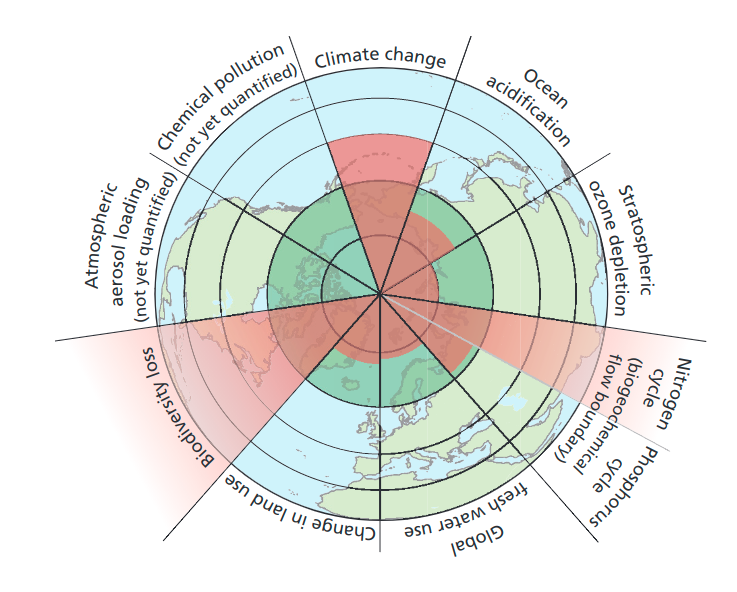
\includegraphics[scale=0.3]{/home/jackreid/Documents/School/Research/Space_Enabled/Thesis/Figures/chap2/Planetary_Boundaries.png}
	\caption[Planetary Boundaries]{Planetary Boundaries. From \cite{rockstromSafeOperatingSpace2009}}
	\label{fig:boundaries}
\end{figure}

While the impacts of these excesses will be felt globally, they will most heavily fall upon some of the poorer and historically oppressed states, harming those with the least capacity of absorb such impacts and thereby potentially exacerbating global inequality. The spatial variation of the estimated impacts of climate change, for instance, can be seen in Figure \ref{fig:vulnerability}.

\begin{figure}[h]
	\centering
	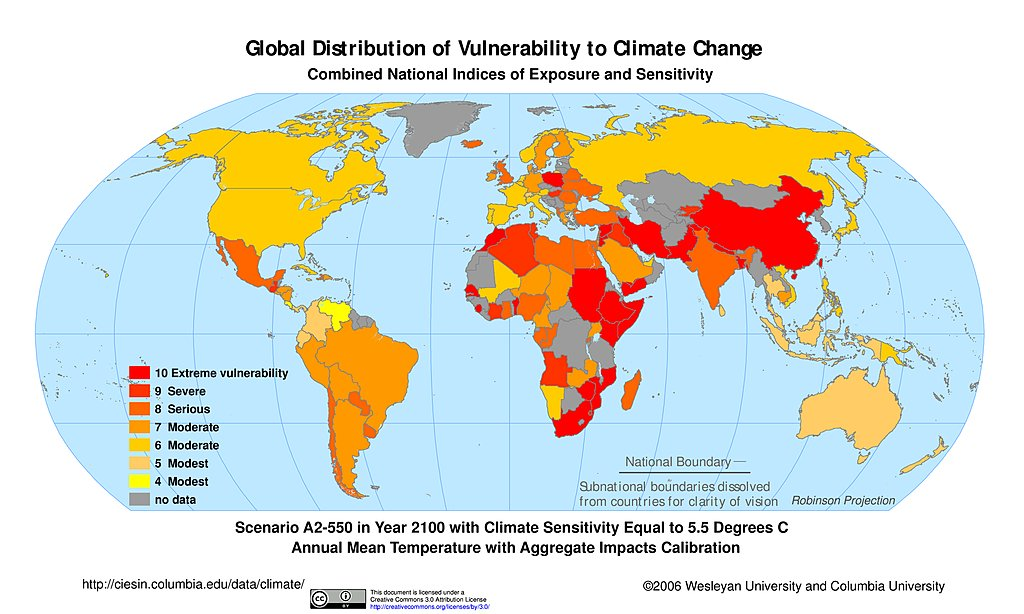
\includegraphics[scale=1.2]{/home/jackreid/Documents/School/Research/Space_Enabled/Thesis/Figures/chap2/vulnerability_map.jpg}
	\caption[Assessment of global distribution of vulnerability to climate change]{Assessment of global distribution of vulnerability to climate change. From \cite{yoheSyntheticAssessmentGlobal2006}}
	\label{fig:vulnerability}
\end{figure}

%Furthermore, as was suggested by the Johannesburg definition of sustainable development, the effects of violating these planetary boundaries will not be limited to a particular domain of human life. Table \ref{table:bau} estimates such multi-domain impacts on different regions of the world iff major, international corrective efforts are not undertaken immediately. The numerous connections between these domains is a key motivation for this work and for the methods chosen, as will be seen later.
%
%\begin{table}[h]
%\begin{minipage}{\textwidth}
%\caption[Estimated impacts of "business-as-usual" by domain and region.]{Estimated impacts of "business-as-usual" by domain and region. H=High; M=Moderate. Adapated from \cite{rockstromSustainableDevelopmentPlanetary2013} and \cite{sachsAgeSustainableDevelopment2015} \protect\footnotemark[1]}
%\label{table:bau}
%\begin{center}
%\tiny
%\begin{tabular}{ | L{2cm} | C{1cm} | C{1cm} | C{1cm} | C{1cm} | C{1cm} | C{1cm} | C{1cm} | C{1cm} | } \hline
%& North America & Latin America \& Caribbean & Europe & Middle East \& North Africa & Sub-Saharan Africa & South \& Central Asia & Southeast Asia \& Pacific & East Asia \\ \hline
%
%Food Insecurity \& Malnutrition & & & & \cellcolor{red!25} H & \cellcolor{red!25} H & \cellcolor{red!25} H & \cellcolor{yellow!25} M  & \cellcolor{yellow!25} M \\ \hline
%
%Poverty & & & & \cellcolor{yellow!25} M & \cellcolor{red!25} H & \cellcolor{red!25} H & \cellcolor{yellow!25} M  & \cellcolor{yellow!25} M  \\ \hline
%
%Land Use Change & & \cellcolor{red!25} H & & & \cellcolor{red!25} H & \cellcolor{yellow!25} M  & \cellcolor{yellow!25} M  & \cellcolor{yellow!25} M  \\ \hline
%
%Soil Degradation & & & & \cellcolor{yellow!25} M  & \cellcolor{red!25} H & \cellcolor{red!25} H   & \cellcolor{yellow!25} M  & \cellcolor{red!25} H   \\ \hline
%
%Water Shortage & \cellcolor{yellow!25} M & & & \cellcolor{red!25} H & \cellcolor{red!25} H & \cellcolor{red!25} H & \cellcolor{yellow!25} M  & \cellcolor{yellow!25} M \\ \hline
%
%Water \& Air Pollution & \cellcolor{yellow!25} M & & \cellcolor{yellow!25} M & \cellcolor{yellow!25} M  & &\cellcolor{red!25} H  & \cellcolor{red!25} H  & \cellcolor{red!25} H \\ \hline
%
%Biodiversity Loss & \cellcolor{yellow!25}  & \cellcolor{red!25} H  & \cellcolor{yellow!25} M & \cellcolor{yellow!25} M  & \cellcolor{yellow!25} M & \cellcolor{yellow!25} M  & \cellcolor{red!25} H  & \cellcolor{red!25} H \\ \hline
%
%Sea Level Rise & \cellcolor{yellow!25} M & \cellcolor{yellow!25} M & \cellcolor{red!25} H & \cellcolor{yellow!25} M & \cellcolor{red!25} H & \cellcolor{red!25} H &\cellcolor{red!25} H  & \cellcolor{red!25} H \\ \hline
%
%Ocean Acidification &  \cellcolor{yellow!25} M & \cellcolor{red!25} H & \cellcolor{red!25} H & \cellcolor{yellow!25} M & \cellcolor{yellow!25} M  & \cellcolor{yellow!25} M & \cellcolor{red!25} H & \cellcolor{yellow!25} M \\ \hline
%\end{tabular}
%\end{center}
%\end{minipage}
%\end{table}
%
%\footnotetext[1]{It should be noted that, despite the latter of these two sources citing the former, the two sources differ in noticeable ways, with no explanation provided in either document. Where they are in conflict, I have chosen to use the latter source. In the former source, there is also a error: Ocean Acidification in the Middle East / North Africa is listed as "H" but the cell is in yellow. The correct entry is not known, so I have gone with "M" in yellow here in order to avoid overstatement.}

A key reason why these planetary boundaries have been so recklessly exceeded despite the enormous human costs that will result is that these aspects of the environment have historically been both undervalued and poorly understood, at least by those championing economic development. Historically, surveys and quantifications of the natural environment focused primarily, or even entirely, on resources that could be extracted and exploited for economic benefit. In early forest surveys, for instance, "Missing... were all those parts of trees, even revenue-bearing trees, which might have been useful to the population but whose value could not be converted into fiscal receipts" \cite{scottSeeingStateHow2020}. Just as these factors were missing from accountings of the natural environment, so were they missing form accounts of human society. "Non-human animals are rarely considered within the realms of social theory, and yet... animals can be regarded as a `marginal social group' that is `subjected to all manner of socio-spatial inclusions and exclusions.'" (\cite{philolAnimalsGeographyCity1995,westcoatBringingAnimalsBack1995,wolchAnimalGeographiesPlace1998}as paraphrased in \cite{harrisRethinkingMapsMorethanhuman2011}). While these authors were referring primarily to animals, it is also  I would argue that this includes plants too, as is particularly evident in the common definition of a weed as a plant growing where it is not wanted.

Fortunately, economists and earth scientists in recent decades have embarked on an effort to better understand and catalog such \textit{ecosystem services}, that is to say, the various benefits that humans are provided by the natural environment and healthy ecosystems in particular. Figure \ref{fig:services_wellbeing} illustrates these connections between the environment and human wellbeing, along with the degree to which these connections are mediated by socioeconomic factors. This work has progressed to the extent that there is now a regularly updated database of almost 5,000 value observations of ecosystem services in a wide variety of regions and biomes (though it should be noted that the database overrepresents valuations involving the United Kingdom, inland wetlands, and coastal systems) \cite{grootEcosystemServicesValuation2020}. Cataloging such ecosystem services is only one step, however. We must also present this data in useful ways to decision-makers  so that they may act upon it, as well has provide them with the tools for them to identify additional, uncataloged ecosystem services in their own communities.

\begin{figure}[h]
	\centering
	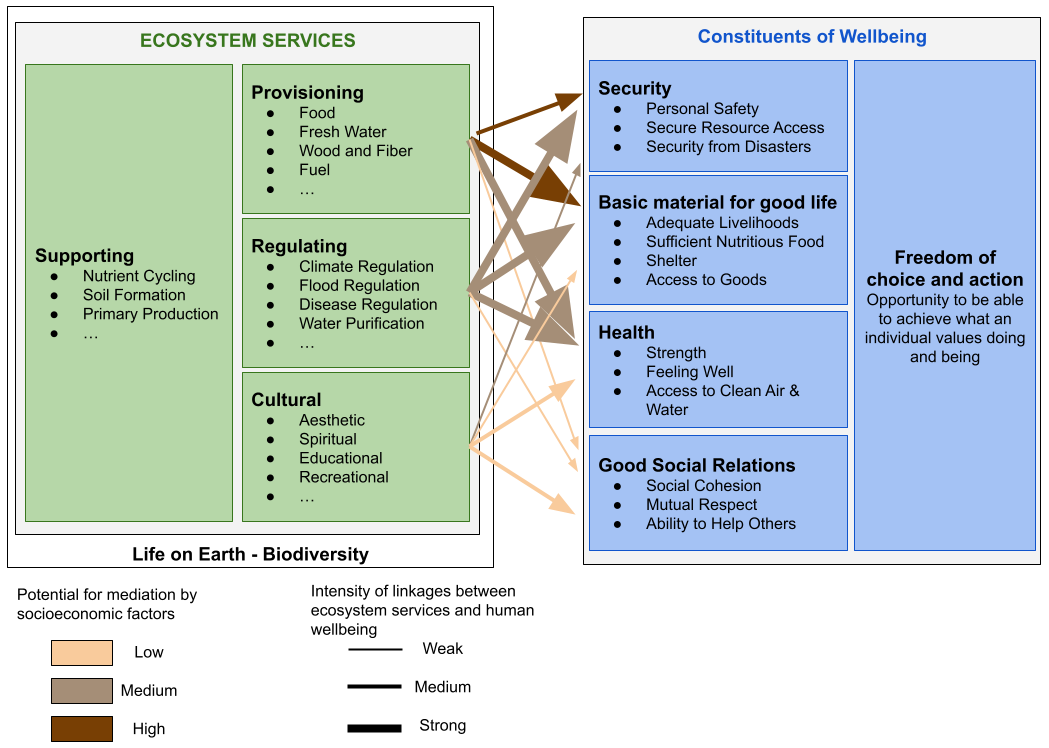
\includegraphics[scale=0.25]{/home/jackreid/Documents/School/Research/Space_Enabled/Thesis/Figures/chap2/services_wellbeing.png}
	\caption[Linkages between categories of ecosystem services and compotents of human wellbeing]{Linkages between categories of ecosystem services and compotents of human wellbeing. Adapted from \cite{reidEcosystemsHumanWellbeing2005}}
	\label{fig:services_wellbeing}
\end{figure}

\subsection{Remote Observation Data} \label{sec:remote}


While many of the initial efforts at remote observation from air and space were done with military objectives in mind, scientific, commercial, and social applications soon became abundant. Since much of space-based remote observation in the past several decades has been primarily driven by large governmental scientific organizations, much of that data has been made publicly accessible. An enormous amount of \ac{eo} satellite data is freely available to the public through 20+ \ac{nasa} earth science satellites \cite{shirahNASAEarthObserving2017}, the \ac{esa} Copernicus Programme (which includes both the 6 Sentinel satellites and in-situ measurements), the various satellites managed by the \ac{jaxa} \ac{eoc}, the \ac{cbers}, and the satellites of other space agencies. 
%
%While this data is largely free currently, this has not consistently been true, nor is it guaranteed to continue in the future \cite{borowitzOpenSpaceGlobal2017}. For most of the early history of satellite observation, imagery was kept highly classified and zealously guarded, to the extent that Congressman George Brown Jr., who was integral in the establishment of the US \ac{ostp}, the \ac{epa}, and the \ac{ota}, resigned from his post on the House Intelligence Panel in protest over the enforced secrecy in even discussing the topic \cite{healyRepBrownQuits1987, barry1992mappings}. Even when the data was available to the public, it was not always freely available, as various countries have made attempts to monitize remote observation data. In the 1970s and early 1980s, for instance, Landsat data was a government-managed operation that provided products at a low-cost, based primarily on the cost of reproduction. In the 1980s, however, the program was transfered to a private entity and prices were increased by more than an order of magnitude and significant copyright restrictions were put in place \cite{mchaffieManufacturingMetaphors1994}. Currently the data is once again made free after the monitization efforts met with limited success \cite{waldropLandsatCommercializationStumbles1987}, but this may not remain the case moving forward \cite{popkinUSGovernmentConsiders2018}.

%The use patterns of remote observation data has varied for reasons beyond cost and military secrecy, however. 

Social applications of remote observation datat were being considered from quite early on. 

%As Jennifer Light recorded, "one proponent [from the last 1940s] explained, photointerpretation data did not directly provide `social data,' yet they were `pertinent to social research needs in so far as such `physical data' have meaningful sociological correlates" \cite{lightWarfareWelfareDefense2005}. In the succeeding decades, the degree to which humans have altered the surface of our planet has only increased and, as a result, we can now also infer a great deal more about humans from images of that surface. 

By the early 1970s five rationales for using satellite imagery in city planing had become widespread \cite{lightWarfareWelfareDefense2005}:

\begin{enumerate}[itemsep=0pt,parsep=0pt]
	\item{It offers a synoptic, total view of the complex system in a given area.}
	\item{Satellites provide repetitive, longitudinal coverage.}
	\item{Satellite inventories were more efficient and up-to-date than ground surveys.}
	\item{Remote sensing was objective.}
	\item{Satellites produced digital imagery that could be easiliy combined with ground-based data in novel \acp{gis}.}
\end{enumerate}

Despite these rationales, or perhaps because of how short reality fell from these rationales at the time, cities and metropolitan areas largely elected not to use satellite imagery for several decades, choosing instead to rely on aerial imagery and ground-based surveys \cite{lightWarfareWelfareDefense2005}. However, much as changed since the 1970s. The rise of multiple \ac{eo} satellite companies, including the company Planet's 100+ satellites \cite{tepperSatelliteMakerPlanet2015}, Digital Global's WorldView satellites, and Astro Digital’s ongoing constellation build-out \cite{shieberAstroDigitalLaunched2017}, suggests that yet more satellite data is soon to be available for a price. These data sources are likely to be complimentary, with the commercial satellites primarily providing visual imagery and \ac{nasa} satellites primarily supplying other forms of scientific data, though the \ac{modis}, the \ac{viirs}, and the Landsat program all capture visual imagery as well. While many of these satellites were designed primarily with scientific purposes in mind, this data is increasingly being used by a wide variety of groups around the world to enable sustainable development and other humanitarian applications, such as  forest fire tracking [via \ac{modis} and \ac{viirs} \cite{schroederNewVIIRS375m2014}], agricultural monitoring [via \ac{gpm} for rainfall \cite{houGlobalPrecipitationMeasurement2014} and GRACE for soil moisture \cite{wahrTimevariableGravityGRACE2004}], climate change vulnerability assessments [via \ac{icesat2} for vegetation and ice monitoring \cite{mcgillMultipleAltimeterBeam2013}], and many other applications, such as the upcoming \ac{swot} \cite{biancamariaSWOTMissionIts2016}.

Furthermore, over the course of the past two decades, efforts have been made to systematize the application of remote sensing data to inform decision-making on a host of sustainable development areas. Internationally, over 100 countries worked together to form \ac{geo} and 60 agencies with active earth observation satellites have formed the \ac{ceos}. In the US, the primary source of such applications is the \ac{nasa} Applied Science Program, a part of the Earth Science Division, that includes programs focused on disasters, ecological forecasting, health \& air quality, water resources, and wildland fires, using data from \ac{nasa} satellites as well as those of the \ac{usgs} and the \ac{noaa}. The Applied Science Program has clearly learned from \ac{nasa} past failures of engagement with local decision-makers, and now publish guides on how to ensure that new projects are actually helpful to users \cite{irwinSERVIRServicePlanning2017}. In keeping with this new mentality, the Applied Science Program, through their Capacity Building portfolio, frequently partners with other organizations, such as \ac{usaid}. For instance, both groups worked together to form the \ac{servir}, which provides geospatial information and predictive models to parts of Africa and Asia. In a similar collaborative effort, \ac{nasa} and \ac{usaid} have also integrated remote sensing data into the \ac{fews}. 

Such efforts have been quite successful in their goals, but have required significant time, expertise, and effort to create and maintain. As overpass frequencies, resolutions, and computational speed have increased, it is increasingly possible to conduct much more rapid, localized, and ad hoc applications of remote sensing data for sustainable development and humanitarian purposes. Within 48 hours and one week respectively, \ac{nasa} was able to provide maps of damaged areas of Mexico City to Mexican authorities following the 2017 earthquake \cite{nasajetpropulsionlaboratorySatelliteRadarDetects2017} and maps of damaged areas of Puerto Rico to the \ac{fema} following Hurricane Maria \cite{nasajetpropulsionlaboratorySatelliteDataPuerto2017} (in fact, both of these maps were provided during the same week), through \ac{nasa}'s Disasters Team under the Applied Sciences Program. Such data collection and processing can increasingly be done without the expertise and remote observation systems of governmental space agencies, as demonstrated by a recent effort to conduct near-real-time deforestation monitoring and response \cite{finerCombatingDeforestationSatellite2018}.

These developments have powerful implications for equity. "The geography agenda is distorted by being data-led... The first law of geographical information: the poorer the country, the less and the worse the data"  (\cite{overton1991further} as paraphrased by \cite{taylorGeographicInformationSystems1994}). Remote observation has the potential to help upend this, by providing at least some base level of data globally, with no distinctions for borders or wealth. Increasingly, sustainable development applications of remote observation data are not limited by available remote observation platforms, but by lack of knowledge by potential end-users of its value and by the tools to make use of available data. While data is often available (either freely or at some cost), it is not always readily accessible (particularly in real time) or easily interpreted. Those with the knowledge and capabilities to access and transform this data continue to reside primarily in government agencies and universities (though we have certainly seen heartening growth of such users in a much more diverse set of countries over the past couple of decades). The majority of prominent \acp{eos} are still designed primarily with scientific, meteorological, or military purposes in mind, limiting their utility in more applied contexts, regardless of the creativity of users. And many successful applications of \ac{eo} data, particularly that which is not straightforward visual imagery, remain squarely focused on characterizing specific, usually environmental, phenomena, such as wildfires \cite{schroederNewVIIRS375m2014},  aquatic bacterial growths \cite{stromingQuantifyingHumanHealth2020}, or deforestation \cite{lagomasinoMeasuringMangroveCarbon2019}, with only limited excursions into assessing the connections between such phenomena and human wellbeing.

More is needed to enable the use of \ac{eo} data for human decision-making in such a way that acknowledges the linkages between the environment and humans. This is major aim of this work. 


\subsection{GIS and Decision Support} \label{sec:gis}

The term \ac{gis} refers to any digital system for storing, visualizing, and analyzing geospatial data, that is data that has some geographic component. It can be used to discuss specific systems, a method that uses such systems, a field of studying focusing on or involving such systems, or even the set of insitutions and social practices that make use of such a system \cite{sheppardGISSocietyResearch1995}. This may seem vague, but due to the diversity of its use, it is difficulty to hammer out a more specific definition without excluding important aspects \cite{goodchildOverviewDefinitionGIS1992, picklesToolScienceGIS1997, chrismanWhatDoesGIS1999, heikkilaGISDeadLong1998}. One perspective, however, is to view \ac{gis} to the underlying computer systems enabling the middle three components of the broader \ac{gisc} methodology, as shown in Figure \ref{fig:boundaries}. In that sense, the work related in this thesis can be seen as an exercise in \ac{gisc} spanning all five components, while the specific software produced for this work are instances of \ac{gis}. 

%It should be noted that this distinction is not commonly made outside of academia, with \ac{gis} commonly being used generically to encompass both \ac{gisc} and \ac{gis}. Along these lines, there being some debate about whether \ac{gis} is best viewed as a scientific field in its own right, or as a mere tool for use in various other fields of science (such as environmental science, economics, etc.) \cite{goodchildGeographicalInformationScience1992,goodchildTwentyYearsProgress2010}. One important aspect of the 
%ac{gisc} perspective that is not included in Figure \ref{fig:boundaries}, is that includes "institutional, managerial, and ethical issues \cite{goodchildGeographicalInformationScience1992}, something that is naturally core to this work. 
%
%The term \ac{gis} and the associated field of study originated in the 1960s and 70s with experimental efforts of the Canda Geographic Information System and the US Bureau of the Census to digitize their demographic and land cover data \cite{goodchildGeographicInformationSystems1994}. It should be noted that these early instances were primarily application, rather than technology driven \cite{goodchildGeographicalInformationScience1992}. The key value of \ac{gis} is that it "allows geographers to integrate diverse types of data over different spatial scales from the regional to the global, while the advanced capabilities of GIS for organizing and displaying these data transform the geographer's view of the world" (\cite{tomlinsonPRESIDENTIALADDRESSGEOGRAPHIC1989} as paraphrased in \cite{vereginComputerInnovationAdoption1994}).
%
%\begin{figure}[h]
%	\centering
%	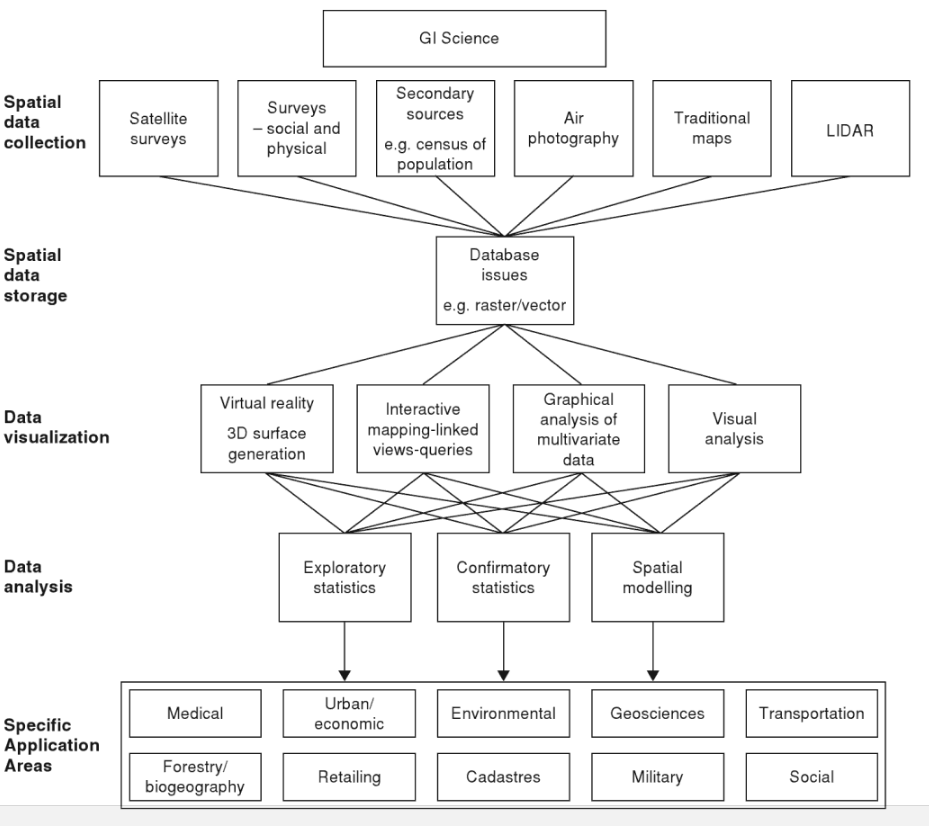
\includegraphics[scale=0.4]{/home/jackreid/Documents/School/Research/Space_Enabled/Thesis/Figures/chap2/GIScience.png}
%	\caption[Overview of Geographical Information Science]{Overview of Geographical Information Science. From \cite{fotheringhamGeographicInformationScience2007}}
%	\label{fig:giscience}
%\end{figure}


%Even with the relatively limited computing capabilities of the era, interest in \ac{gis} grew quickly with local governments quickly adopting it for planning purposes, as was mentioned in Section \ref{sec:remote}. One key moment in the development of \ac{gis} as we know it, was ESRI's creation of the shapefile format (which links geometries with data in a standardized, if somewhat limited, fashion) in the late 1980s, and, more importantly, their open publishing of the format, allowing others to create and manipulate such files \cite{goodchildModelingEarth2011}. In 1990, Tomlin defined the sub-discipline of \ac{gis} known as cartographic modeling, which attemps to generalize and standardize the analytic and synthetic capabilities of geopgrahical information systems. It does so by decomposing data, data-processing tasks, and data-processing control notation into elementary components that can be recomposed with relative ease and great flexibility" \cite{tomlinGISCartographicModeling2012}. This theory would come to underly much of research and development work done with \ac{gis}. including that of this thesis. 

By 1991, Maguire et al. felt that "it is not fanciful to suggest that by the end of the century GIS will be used every day by everyone in the developed world for routine operations" \cite{maguireGeographicalInformationSystems1991}. This, of course, would turn out to be an understatement, as the world is currently incredibly dependent on \ac{gis}. Individuals rely upon the various map applications that we use to search and navigate our world. Governments use maps to visualize their jurisdictions and motivate action, as Chicago has done by visualizing food deserts and mapping where new supermarkets are both needed and economically viable \cite{goldsmithResponsiveCityEngaging2014}. Since the turn of the millenium, spatial data has become deeply ingrained economics, urban studies, private industry, social networks, environmental science, public health, criminal justice, and more \cite{goodchildSpatiallyIntegratedSocial2000}.

%There is now a well established marketplace for geographic data (as shown in \ref{fig:marketplace}) and thus for \acp{gis} to handle that data. It should be noted that the institution that I am associated with, a university, is classified here as a "value-added intermediary" which serves an important connective role between suppliers, infrastructure, and users. This positioning is crucial to the nature of this work, as will be discussed further in Section \ref{sec:plan}. For now it is enough to understand that, whether one is interested in remote observation data or local economics, the question is not whether one should use \ac{gis}, but how. To this end, the next two sections will go into more detail about two different veins of \ac{gis}: collaborative systems and decision support systems.
%
%\begin{figure}[h]
%	\centering
%	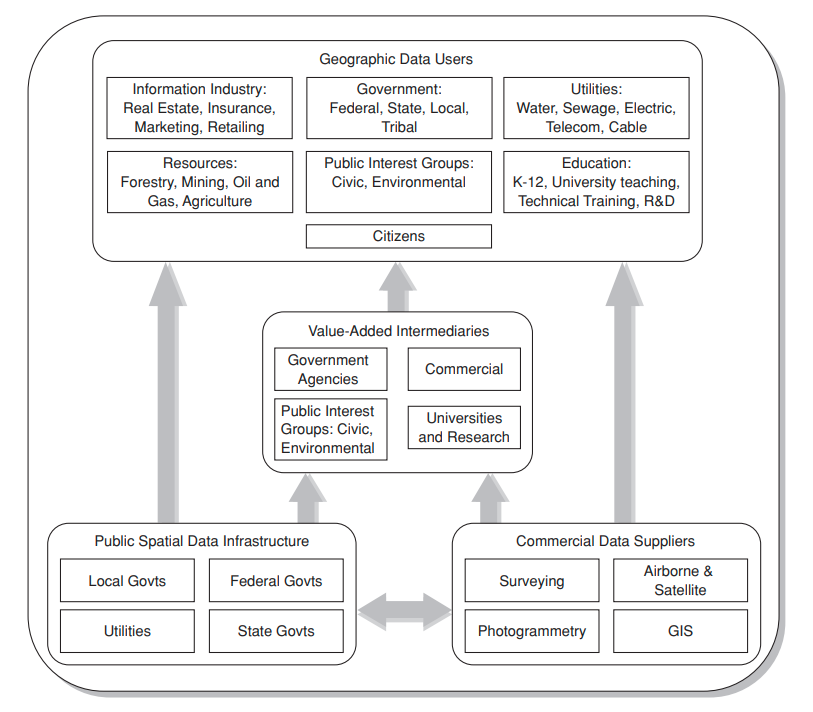
\includegraphics[scale=0.4]{/home/jackreid/Documents/School/Research/Space_Enabled/Thesis/Figures/chap2/GISMarketplace.png}
%	\caption[The marketplace for geographic data]{The marketplace for geographic data. From \cite{cowenAvailabilityGeographicData2007}}
%	\label{fig:marketplace}
%\end{figure}

\subsection{Collaborative and Open Source} \label{sec:collaborative}

Many of the early applications of remote observation data were technology, rather than need, driven. So it was with the closely related field of \ac{gis} as well, leading to powerful critiques by Pickles and others \cite{picklesGroundTruthSocial1994}. These critiques resulted in a reconsideration of the top-down nature of the field and the identification of several potent reasons for broadening the base of participation. First, there was the recognition that the developer of a \ac{gis} is not the supreme authority on all fields. "It is the geomorphologist who is best able to choose the data model for representation of terrain in a GIS, not the computer scientist or the statistician, and it is the urban geographer who is best able to advice on how to represent the many facets of the urban environment in a GIS designed for urban planning" \cite{goodchildGeographicInformationSystems1994}. This means that, while collaborations certainly can introduce additional difficulties, such as cultural conflicts, issues of interpersonal trust, effort required to establish rules and norms of participation, they are also immensely rewarding and can improve the results of the work \cite{tullochInstitutionalGeographicInformation2007}. 

%The dynamics at play in such collaborations can be seen in Figure \ref{fig:east2}. This is certainly a more complicated situation than the traditional, straightforward, academic implementation of a \ac{gis} project.
%
%\begin{figure}[h]
%	\centering
%	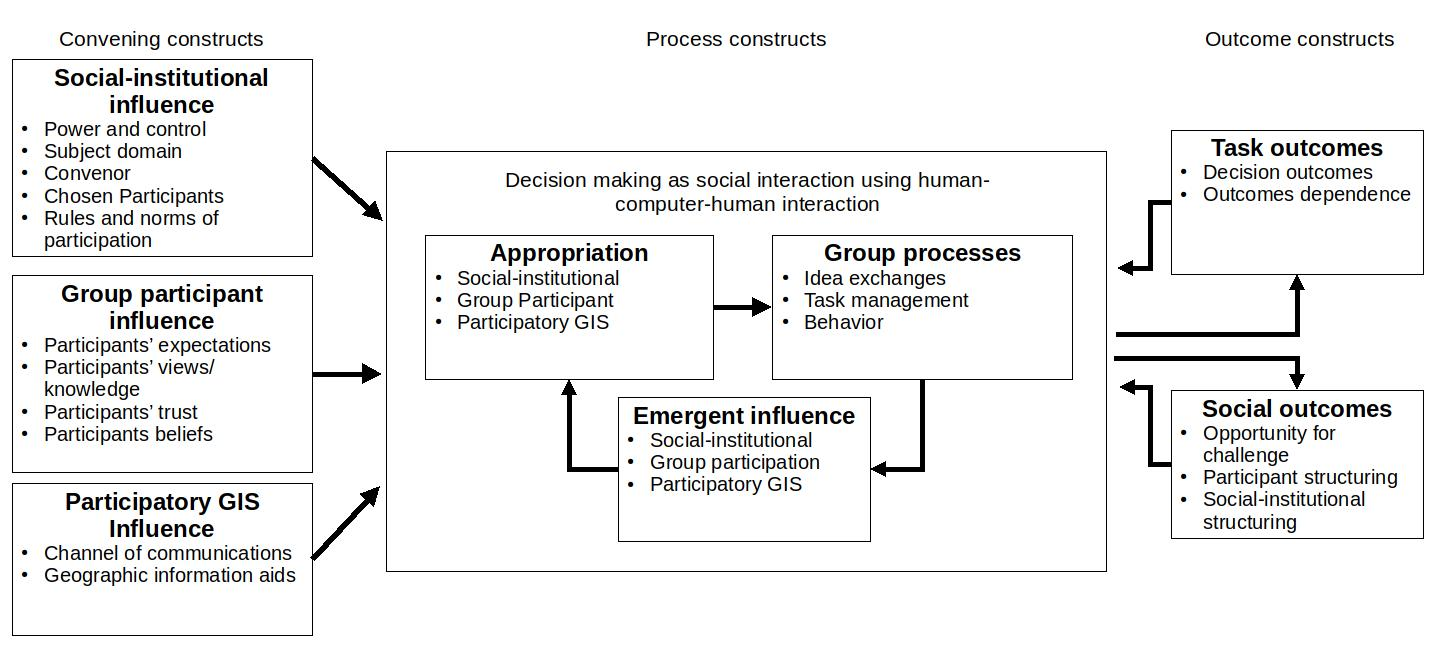
\includegraphics[scale=0.4]{/home/jackreid/Documents/School/Research/Space_Enabled/Thesis/Figures/chap2/east2.jpg}
%	\caption[Enhanced Adaptive Structuration Theory 2 (EAST2)]{Enhanced Adaptive Structuration Theory 2 (EAST2). Adapted from \cite{jankowskiGISGroupDecision2001}}
%%	\label{fig:east2}
%\end{figure}

Second, there was a recognition of the equity concerns at play. Users and disadvantaged communities needed to be involved in the development of \ac{gis} data, analysis, and use, if they were going to have a meaningful chance of improving their circumstances \cite{talenBottomUpGIS2000}. The Canadian International Development Research Centre noted that, "It is impossible to have sustainable and equitable development without free access to reliable and accurate information" \cite{benmouffokInformationDecisionMaking1993}. Meanwhile, academic geographer Matthew Edney argued that, "Without equitable access to GIS data and technology, small users, local governments, nonprofit community agencies, and nonmainsream groups are significantly disadvantaged in their capacity to engage in the decision-making process" (\cite{edney1991strategies} as paraphrased in \cite{harrisPursuingSocialGoals1994}). 

There was thus reason to seek ways to overcoming the limitations of the technology which, as was common sentiment at the time, meant that "for billions the possibility of accessing the best technology and information made available through digital communications network will always be a luxury. Cartographic information, digital or otherwise, becomes a commodity in its mass production and marketing" \cite{mchaffieManufacturingMetaphors1994}. 

In the early 2000s, this desire motivated the growth in interest towards deconstructing current practices and expanding participation. Several names and frameworks were proposed, including Bottoms Up GIS \cite{talenBottomUpGIS2000}, critical cartography \cite{cramptonIntroductionCriticalCartography2005, kimCriticalCartographyParticipatory2015}, GIS and Society \cite{sieberPublicParticipationGeographic2006}, and \ac{ppgis}. The last of these, which sought to directly involve the public, would become the most widely used, and would be associated with the broader field of \ac{pgis} \cite{sieberPublicParticipationGeographic2006}, which also included other stakeholders, including government officials, \acp{ngo}, private corporations, etc. It should be noted that these fields seek involvement in both the production of data and in its application, not merely one or the other \cite{weinerParticipatoryGeographicInformation2007, talenBottomUpGIS2000}. For example, in Washington state in 2002, several American Indian tribes were using \ac{gis} technology to "inventory, analyze, map, and make descisions regarding tribal resources... includ[ing] timber production, grazing and farm land, water rights, wildlife, native plants, cultural sites, environmental data and hazardous site monitoring, historical preservation, health and human resources" \cite{bondCherokeeNationTribal2002}. And in 1999, the 'What If?' \ac{pss} was created to use "GIS data sets that commnities have already developed to support community-based efforts to evaluate the likely implications of alternative public-policy choices" \cite{klostermanWhatIfCollaborative1999}. 

%This dual involvement promotes, as Michael Curry put it, both "knowing \textit{how}" (the "ability to do something") and "knowing \textit{that}" (the "knowledge about how something works") \cite{curryGeographicalInformationSystems1994}. Having only the former forces the user to rely upon blind trust, instilling a sense of complacency or alieanation and preventing creativity. Knowing only the latter, enables discourse about a topic but prevents the user from actually implementing new ideas. It is only with both together that a person becomes a true participant in a field and make their own choices. This is important as expansion of choice is valuable for both intrinsic (for its own sake) and instrumental (to attain preferred positions) reasons \cite{senFreedomChoiceConcept1988}.

\ac{pgis} has thus naturally been strongly advocated and widely adopted over the past three decades \cite{drummondFutureGISPlanning2008}, with numerous frameworks being proposed for how to implement it \cite{brommelstroetPlanningSupportSystems2010}. 

%A relatively early project in this vein, for example, sought to try and overcome issues of inequal access and use of \ac{gis} technology in South Africa in the early 1990s through the pursuit of five specific objectives \cite{harrisPursuingSocialGoals1994}: 
%
%\begin{enumerate}[itemsep=0pt,parsep=0pt]
%	\item{Enhanced community/development planner interaction in a research and policy agenda setting}
%	\item{The integration of local knowledge with exogenous technical expertise.}
%	\item{The spatial representation of relevant aspects of local knoweledge.}
%	\item{Genuine community access to, and use of, advanced technology for rural land reform.}
%	\item{The education of "expert" rural land use planners about the importance of popular participation in policy formulation and implementation.}
%\end{enumerate}

%Such objectives are common across \ac{pgis} projects and the success of this pursuit has come to be recognized even by many entrenched institutionalists. The former vice-mayor of New York City, for instance, argues that digital \ac{gis} tools that provide open data (1) free data from bureaucractic constraints, allowing real time combination of data from different souces; (2) construct a loop between government and the community in which cooperation builds respect continuously; (3) enable two-way communication, promotiving collaboration \cite{goldsmithResponsiveCityEngaging2014}. That said, some of these implementations have been criticized for being participative in name only, particularly within the research domain \cite{tebrommelstroetRelevanceResearchPlanning2009}.

%Civic technology \cite{poppertNavigatingFieldCivic2021}

Many \ac{pgis} implementations still rely upon closed source, proprietary code for the underlying software \cite{heikkilaGISDeadLong1998}. Participants made have been able to generate new data and perform analyses, but they often could not access the code itself or change the models directly. This was due to a combination of factors: limited diffusion of programming knowledge; a limited selection of software tools, many of which were closed source; limited access to computers and the internet; and limited collaboration tools, particularly for geographically distributed collaborations \cite{cramptonIntroductionCriticalCartography2005}. Over the past couple decades however, all three of these limitations have been greatly mitigated (though not eliminated), due to the growth of the internet and the related diffusion of programming knowledge and rise of the open source movement. As two leaders of the \textit{theirwork} \ac{ppgis} project in 2011 put it \cite{williamsonTheirworkDevelopmentSustainable2011}, 

\blockquote{The open source movement at its core stands for the development of source code... in a completely open and free way. Pragmatically, this manifests itself as a methodology of making code freely available to anyone who may wish to access it for any purpose, unconditionally. Concurrently, open source is for many a philosophical approach to software development, and is see as the only truly sustainable approach to software development... In both its execution as a model for making possible new forms of collaborative work, and its philosophical underpinnings of sustainability and openness, it is an essential component in and fluence upon a computer-based mapping solution.}

This passionate call for open source software is about more than a philosophical ethical stance. It is also about enabling critique and improvements. "Map studies needs to open the `black boxes' of mapping software, to start to interrogate algorithms and databases, and in particular to investigate the production of ready-made maps that appear almost magically on the interfaces of gadgets and devices we carry and use everyday, often without much overt thought about how they work and whose map they project onto their interface" \cite{dodgeMappingModesMethods2011}.

It should be noted that some work has placed the responsibility for limited adoption of \ac{gis} tools on the planners/users themselves, specifically their lack of will and training with the tools \cite{gocmenBarriersGISUse2010}. While this may be the case, this lack of will and training is almost certainly itself due to a lack of outreach on behalf of the tool developers, and thus \ac{pgis} is still reasonable strategy to address these barriers.	 


%\subsubsection{Why Scenario Planning and Decision Support?}
%
%
%Planning can be defined as "the premeditation of action, in contrast to management [which is] the direct control of action" \cite{harrisLocationalModelsGeographic1993}. In general, planning tends to concern itself with more long-term affairs that management does, during which it strives for the "avoidance of unintended consequences while pursuing intended goals." Models, and their specific implementations as decision/planning support tools, are one means of achieving this.

%As late as 1990, many researchers were arguing that \ac{gis} was not mature enough to serve as the basis for a \ac{dss} \cite{jankowskiIntegratingGeographicalInformation1995}.
%
%Börjeson et al. propose three different kinds of scenario generation: predictive, explorative, and normative \cite{borjesonScenarioTypesTechniques2006}, with most urban planning applications focussing on the normative type \cite{avinUsingExploratoryScenarios2020}. Maier et al. built upon this to provide a framework for how to handle varying degrees of uncertainty in scenario planning \cite{maierUncertainFutureDeep2016}. 
%
%
%Harris and Batty defined two principle requirements of planning support systems \cite{harrisLocationalModelsGeographic1993}:
%\begin{enumerate}[itemsep=0pt,parsep=0pt]
%	\item{The search for good plans take place through informed trial and error, since system optimization is impossible.}
%	\item{The tool must be able to trace out the consequences of alternatives, as this is the primary means of comparing alternatives.}
%\end{enumerate}
%
%They also define some other relevant requirements to this work \cite{harrisLocationalModelsGeographic1993}:
%\begin{itemize}[itemsep=0pt,parsep=0pt]
%	\item{The tool should be available to public use, including methods and data.}
%	\item{The tool should acommmodate research and adaptation.}
%	\item{The tool should be self-teaching, within reason.}
%	\item{The tool should be adaptable, including to a wide variety of situations, levels of information, etc.}
%	\item{The tool should be built on models and methods that are understandable to the user.}
%\end{itemize}
%
%
%
%
%
%Levels of decision support \cite{jankowskiGISGroupDecision2001}:
%
%\begin{enumerate}[itemsep=0pt,parsep=0pt]
%	\item{\textit{Basic information handling support}}
%%	\vspace{-5mm}
%		\begin{enumerate}[itemsep=0pt,parsep=0pt,topsep=0pt, partopsep=0pt]
%			\item{Information management}
%			\item{Visual aids}
%			\item{Group collaboration support}
%		\end{enumerate}
%%	\vspace{-5mm}
%	\item{\textit{Decision Analysis Support}}
%%	\vspace{-5mm}
%		\begin{enumerate}[itemsep=0pt,parsep=0pt,topsep=0pt, partopsep=0pt]
%			\item{Option modeling}
%			\item{Choice models}
%			\item{Structured group process techniques}
%		\end{enumerate}
%%	\vspace{-5mm}
%	\item{\textit{Group reasoning support}}
%%	\vspace{-5mm}
%		\begin{enumerate}[itemsep=0pt,parsep=0pt,topsep=0pt, partopsep=0pt]
%			\item{Judgement refinement/amplification techniques}
%			\item{Analytical reasoning methods}
%		\end{enumerate}
%\end{enumerate}
%
%
%"Scenario planning is a method of long-term strategic planning that creates representations of multiple, plausible futures of the system of interest." It arose in military and corporate strategies \cite{goodspeedScenarioPlanningCities2020} 
%
%Scenario Planning arose from two independent sources: Herman Kahn at the RAND Corporation working for the Air Defense System Missile Command and Gaston Berger at the Centre d'Etudes Prospectives \cite{bradfieldOriginsEvolutionScenario2005}. These in turn were further developed in the private sector by Shell and GE, with the former publishing more openly on the topic. Numerous forms of scenario planning exist. For instance, Kahn's original forumation was probabilistic, focusing on the most likely scenarios. Berger's, on the other hand, was normative, focusing on the scenarios to be aimed for. Lastly, Shell's has eschewed both of these, focusing instead on capturing a range of potential future scenarios and using them to explore responses and to educate decision-makers.Regardless of the focus, scenario planning centers around the construction of some number discrete "future worlds" that consist of a set of both quantitative and qualitative parameters. Impact on the organization and potential responses are then explored. While the exact methodology varies and different organizations use scenario planning for different purposes, most private corporations use it primarily for long range business planning \cite{bradfieldOriginsEvolutionScenario2005}. That said, scenarios planning has also been used to construct early warning systems, by identifying the important areas and trends to monitor to inform decision-making \cite{tessunScenarioAnalysisEarly1997}.
%
%"A scenario-based strategic plan is... appropriate for vision, framework, comprehensive, system, and redevelopment plans and for those with long time horizons and low or moderate detail" \cite{goodspeedScenarioPlanningCities2020}. 
%
%\textit{Oregon Scenario Planning Guidelines} proposes a six-step process for scenario planning ( \cite{oregonsustainabletransportationinitiativeScenarioPlanningGuidelines2017} as paraphrased by \cite{goodspeedScenarioPlanningCities2020}:
%
%\begin{enumerate}[itemsep=0pt,parsep=0pt]
%	\item{Create a framework for the scenario planning process.}
%	\item{Select evaluation criteria.}
%	\item{Set up for scenario planning: evaluation tools ,data, and building blocks.}
%	\item{Develop and evaluate base-year conditions and reference case.}
%	\item{Develop and evaluate alternative scenarios}
%	\item{Select the preferred scenario}
%\end{enumerate}
%
%Zapata and Kaza provide evidence that scenario planning, particularly when incorporating diverse participants, can help planners cope with significant levels of uncertainty about the future (though they also note that few programs actually involve diverse participants) \cite{zapataRadicalUncertaintyScenario2015}.
%
%Goodman describes four primary kinds of planning support models \cite{goodspeedScenarioPlanningCities2020}: 
%
%\begin{enumerate}[itemsep=0pt,parsep=0pt]
%	\item{Generic Systems Models: Developing a typically non-spatial abstract representation of a system and analyzing how it functions. System dynamics is a classic example.}
%	\item{Economic and Demographic Models: The set of techniques that focus on changes in employment of particular sectors and in populuation of different characteristics. Klosterman is the classic text on these methods. \cite{klostermanCommunityAnalysisPlanning1990}}
%	\item{Place-Type Development and Analysis: Tools used to simulate future outcomes based on land use, zoning, population density, etc. CommunityViz is an example of this \cite{walkerPlannersGuideCommunityViz2017}.}
%	\item{Urban Systems Models: Essentially a combination of generic systems modeling and place-type development and analysis models to accurately represent spatial phenomena over time, such as transportation networks and organic growth. Examples include cellular automata and spatial interaction models.}
%\end{enumerate}
%
%
%Jankowski and Nyerges lay out seven common design requirements for spatial decision support tools \cite{jankowskiGISGroupDecision2001}:
%
%\begin{enumerate}
%    \setlength{\itemsep}{0pt}%
%    \setlength{\parskip}{0pt}%
%	\item{A spatial decision support system for collaborative work should offer decisional guidance to users in the form of an agenda.}
%	\item{A system should not be restrictive, allowing the users to select tools and procedures in any order.}
%	\item{A system should be comprehensive within the realm of spatial decision problems, and thus offer a number of decision space exploration tools and evaluation techniques.}
%	\item{The user interface should be both process-oriented and data-oriented to allow an equally easy access to task-solving techniques, as well as maps and data visualization tools.}
%	\item{A system should be capable of supporting facilitated meetings and hence, allow for the information exchange to proceed among group members, and between group members and the facilitator. It should also allow space- and time-distributed collaborative work by facilitating information exchange, electronic submission of solution options, and voting through the internet.}
%	\item{A system functionality should include extensive multiple criteria evaluation capabilities, sensitivity analysis, specialized maps to support the enumeration of preferences and comparison of alternative performance, voting, and consensus building tools.}
%	\item{A system should provide ncessary functionality to support needs of an advanced user without overwhelming a novice who needs a user-guiding interface.}
%\end{enumerate}
%
%\ac{pgis}: Refer to macro-micro framework from Table 2.1, pg.17. What parts this thesis covers and what parts we envision EVDT covering in the long term.
%
%\begin{table}[h]
%\caption[Generic macro-micro, participtory decision strategy]{Generic macro-micro, participtory decision strategy. Adapted from \cite{jankowskiGISGroupDecision2001}}
%\label{table:macro-micro}
%\begin{center}
%\begin{tabular}{ L{3cm} L{4cm}  L{4cm} L{4cm}} \hline
%& \multicolumn{3}{c}{\textit{Macro-phases in a decision strategy}}  \\ \cline{2-4}
%
%\textit{Micro-activities in a decision strategy} & \textbf{\textit{1. Intelligence}} about values, objectives, and criteria & \textbf{\textit{2. Design}} of a set of feasible options &  \textbf{\textit{3. Choice}} about recommendations \\ \hline
%
%\textbf{A. Gather...} & issues to develop and refine \textbf{value trees} as a basis for objectives & \textbf{primary criteria} as a basis for option generation & \textbf{values, criteria, and option list scenarios} for an evaluation \\ \hline
%
%\textbf{B. Organize...} & \textbf{objectives} as a basis for criteria and constraints & and apply approaches(es) for \textbf{option generation} & approaches to \textbf{priority and sensitivity analyses} \\ \hline
%
%\textbf{C. Select...} & \textbf{criteria} to be used in analysis as a basis for generating options & the \textbf{feasible option list} & \textbf{recommendation} as a prioritized list of options \\ \hline
%
%\textbf{D. Review...} & criteria, \textbf{resources, constraints,} and \textbf{standards} & \textbf{option set(s)} in line with resources, constraints, and standards & \textbf{recommendation(s)} in line with original \textbf{value(s), goal(s),} and \textbf{objectives} \\ \hline
%
%\end{tabular}
%\end{center}
%\end{table}


\subsection{Systems Engineering} \label{sec:se}

Systems engineering is an interdisciplinary approach and means to enable the realization of successful systems. It focuses on holistically and concurrently understanding stakeholder needs; exploring opportunities; documenting requirements; and synthesizing, verifying, validating, and evolving solutions while considering the complete problem, from system concept exploration through system disposal \cite{systemsengineeringbodyofknowledgeSystemsEngineeringGlossary2021}. Something missing from this definition is that systems engineering refers to a specific intellectual tradition that arose out of mechanical, civil, electrical, and aerospace engineering fields in the early-to-mid 20th century. It thus tends to draw from an engineering mindset and relies upon engineering techniques, rather than those of urban planning, architecture, or program management. This is important because the nature of systems engineering is that it is inherently abstracted from its subject matter to a certain degree. The tools of systems engineering were developed in order to design hydroelectric dams, rockets, global communications systems, and much more. In this way it is similar to control theory, in that is is not deeply tied to the specific thing being designed or controlled, only to an abstract understanding of its mechanics and relationships. This means that systems engineers, like some physicists, can have a tendancy to see any problem, any situation, as tractable with a systems engineering perspective.

There is a long history of applying systems engineering techniques to development concerns. US Vice President Herbert Humphrey said in 1968 that "The techniques that are going to put a man on the Moon are going to be exactly the techniques that we are going to need to clean up our cities" \cite{lightWarfareWelfareDefense2005}. In the same year, the RAND Corporation established a multi-year attempt to bring systems analysis and engineering to urban planning. Around the same time, the \ac{aiaa} hosted meetings on urban technologies to bring aerospace expertise to bare on the urban crises of the time \cite{lightWarfareWelfareDefense2005}. It was a heady time, with engineers themselves feeling "that, having reached the moon, they could now turn their energies to solving the problem of growing violence in cities along with other urban "crises" \cite{mazza2017}. 

%These applications were justified by several different rationale, chief among them were \cite{lightWarfareWelfareDefense2005}: 
%
%\begin{itemize} \setlength{\itemsep}{0pt} \setlength{\parskip}{0pt} 
%	\item{Computer simulations and related techniques were simply advances on the statistical models already widely used by the urban planning profession.}
%	\item{The rise of cybernetics, with its cross-disciplinary control analogies, promised to unify disparate fields within urban planning and analysis, resulting in a unified understanding of cities.}
%	\item{The use of these military innovations would transform urban planning and decision-making into scientific endeavors.}
%\end{itemize}

Almost immediately, however, such grand ideas met with difficulties. While recounting the full history of this trajectory is beyond the scope of this work, one can get a sense of it in quotations from urban planners of the time and since:

\blockquote{The systems engineers bring some expertise and substantial pretensions to the problems of the city. Their prinicpal system expertise seems to be relative to complex organizations that are mission oriented. There is in any case a good deal of difference between the mission of reaching the moon, and the mission of surival and welfare for soceity and the city. The systems engineer can in general deal best with subsystems and specific tasks, and he therefore suboptimizes. This is a charitable description. \cite{robinsonDecisionmakingUrbanPlanning1972}}

\blockquote{Trying to solve `earthly problems,' especially urban problems through aerospace innovations had shown that `transporting the astronauts from terra firma to land on the lunar sphere, travel hither and yon over its surface, and then back home to Houston' was a comparatively simple task. \cite{lightWarfareWelfareDefense2005}}

Ultimately, reality fell far short of both hopes and expectations, for a host of reasons examined in the literature. \cite{lightWarfareWelfareDefense2005, mazza2017, eubanksAutomatingInequalityHow2018, scottSeeingStateHow2020, mcloughlinSystemGuidanceControl1972, mcloughlinChartingPossibleCourses1972}. This led to the gradual rejection and retreat of systems engineering in development planning. As early as 1973, planning scholars were (perhaps preemptively) eulogizing the death of large-scale models and other tools of the systems engineer \cite{leejrRequiemLargeScaleModels1973}. The intervening decades have seen the fields of systems engineering and development planning grow largely independently of one another. Since the 1970s, the urban planning professional has evolved and adopted computational models on their own terms. Interactive \ac{dss} abounds \cite{waddellUrbanSimModelingUrban2002, walkerPlannersGuideCommunityViz2017}. The use of \ac{gis} has become the norm \cite{jankowskiGISGroupDecision2001,tomlinGISCartographicModeling2012,wilsonHandbookGeographicInformation2007}., including more participatory variants \cite{sieberPublicParticipationGeographic2006}. Numerous quantative economic and social indeces have been developed \cite{boyceFrameworkDefiningApplying1972, cliftonQuantitativeAnalysisUrban2008,readAssetbasedEconomicDevelopment2012,sawickiNeighborhoodIndicatorsReview1996,valRegionalLocalEconomic1991} . Mathematical tools such as cellular automata have become popular \cite{battyCitiesComplexity2005,laufUncoveringLanduseDynamics2012}. Digital models underly the popular subdiscipline of scenario planning \cite{goodspeedScenarioPlanningCities2020,zapataRadicalUncertaintyScenario2015}. Interdisciplinary, integrated models have even started to re-emerge \cite{millerIntegratedUrbanModeling2018,moeckelTrendsIntegratedLanduse2018,shahumyanIntegrationLandUse2017}. 
Arguably urban planning has adopted many of the tools and methodologies of systems engineering.

At the same time, systems engineering has changed. The belief that systems, even human systems, can be made simple, rational, and controllable has been largely outmoded within the field. Instead, in the guise of theories of complex systems and chaos, they have adopted Jane Jacob's view that ``intricate minglings of different uses are not a form of chaos. On the contrary they represent a complex and highly developed form of order." \cite{jacobsDeathLifeGreat2016}. Complex systems, emergence, systems-of-systems, and complex adaptive systems have all become popular fields of study within systems engineering \cite{mcdermidComplexityConceptCauses2000,sussmanTeachingComplexSociotechnical2010, chenComplexityEmergenceEngineering2009,deguetElementsEmergenceIssue2006,
officeofthedirectorofsystemsandsoftwareengineeringSystemsEngineeringGuide2008,glassComplexAdaptiveSystems2011,
incosecomplexsystemsworkinggroupComplexityPrimerSystems2016,bradleyComplexSystemGovernance2016,
mittalHumanLoopSystem2015,sheardPracticalApplicationsComplexity2005}, with numerous frameworks being proposed for how to classify and handle such systems \cite{kurtzNewDynamicsStrategy2003,martinFrameworkQuantifyingComplexity2004, sheardComplexityTypologySystems2010, righiCharacterizingComplexitySociotechnical2012,schottlQuantifyingComplexitySocioTechnical2015, reymondetFrameworkSenseMakingComplex2016}. Faced with such systems, engineers have had to recognize their own inability to definitively predict the future and have turned to probabalistic methods that instead ``manage" complexity over longer time scales, such as epoch-era analysis \cite{rossUsingNaturalValueCentric2008,vascikMethodExploringProgram2015} (which in many ways resembles the aforementioned urban planning method called scenario planning).

Parallel to this, systems engineers have moved away from singlemindedly implementing the directives of an individual client to identifying, mapping, and analyzing the stakeholders in a system and their connections to one another in order to inform the design of the system. This stakeholder analyses involves both qualitative and quantitative tools, such as the Stakeholder Requirements Definition Process \cite{incoseINCOSESystemsEngineering2015}, Stakeholder Value Network Analysis \cite{fengDependencyStructureMatrix2010a}, and qualitative interviews of representatives from different stakeholder groups (something that would have been anathema to the earlier era of systems engineering. In order to translate these complicated networks of stakeholders into designs, systems engineers have developed methods for handling multi-stakeholder negotiation and \cite{fitzgeraldEffectsEnhancedMultiparty2015,fitzgeraldRecommendationsFramingMultistakeholder2016,weckMULTISTAKEHOLDERSIMULATIONGAMING2012} tradespace visualization and exploration \cite{fitzgeraldEffectsEnhancedMultiparty2015,fitzgeraldRecommendationsFramingMultistakeholder2016,groganInteractiveModelsSystem2015,rossMultiAttributeTradespaceExploration2004,selvavaleroRulebasedSystemArchitecting2012}, , the latter of which demonstrates an increased willingness to appreciate the psychology and experience of ther user. The historic preference of the impersonal and `objective' versus the personal and `subjective' is by no means unique to systems engineering. It can also be found in economics, jurisprudence, education theory, political science, and even moral philosophy \cite{banuriModernatizationItsDiscontents1990}. The development of stakeholder analysis has helped to bridge the gap between these two and thus rectify this traditional deficiency. In fact, the use of stakeholder analysis in contemporary systems engineering is, in a way, a step away from the worldview that sees ``human beings as unknowable black boxes and machines as transparent," a viewpoint that "surrenders any attempt at empathy and forecloses the possibility of ethical development" and is a tacit ``admission that we have abandoned a social commitment to try and understand each other" \cite{eubanksAutomatingInequalityHow2018}.

All of this suggests that the fields of systems engineering and urban planning are perhaps more close to each other than ever before, even showing some elements of convergent evolution (see the use of the term complex adaptive system in both fields \cite{yamuAssumingItAll2016}). Much benefit could be gained through more direct dialogue and collaboration with one another. Why then, do we not see that occuring? After all, several of the critical comments made about systems engineering cited above were from recent years. Part of this is likely historical memory. While decades have elapsed, we are still within a single professional lifetime of some of the excesses of systems engineering. But some concerns can be found much temporally closer. While urban planning is a deeply historical field, systems engineering is not. What histories do exist tend to focus on the engineered technical systems, such as the Apollo program \cite{brillSystemsEngineeringRetrospective1998}, rather than the planning dalliances of the 50s-70s. This is has not gone unnoticed: ``One cannot know about the history of media stereotyping or the nuances of structural oppression in any formal, scholarly way through the traditional engineering curriculum of the large research universities from which technology companies hire across the United States. Ethics course are rare" \cite{nobleAlgorithmsOppressionHow2018}. This can lead to each new generation of engineers using new tools that are attempts to resolve the mistakes of the past, but while maintaining the same tabula rasa mindset that led their forebearers astray. Can one begrudge the urban planner their skepticism when one of the highest profile contemporary applications of systems engineering to planning is the `urban digital twin' or `smart city' \cite{goldsmithResponsiveCityEngaging2014,sregantanSingaporePipsLondon2018, franciscoSmartCityDigital2020,ruohomakiSmartCityPlatform2018, gohBuildingSingaporeDigital2015} that seems to be a repitions of the belief that ``complex controversies can be solved by getting correct information where it needs to go as efficiently as possible," that ``political conflict arises primarily from a lack of information," and that ``if we just gather lack the facts, systems engineers assume, the correct answers to intractable policy problems like homelessness will be simple, uncontroversial, and widely shared" \cite{eubanksAutomatingInequalityHow2018}. This work seeks to chart a different, more history-cognizant path, and thereby capture some of the potential benefit of systems engineering in the sustainable development domain without running afoul of the classic blunders.


Sustainable development is a pressing need for our world, one that we need our best minds and methods to fulfill. Systems engineering, particularly the new, humbler systems engineering, is well posed to contribute, provided it can maintain that humility. Opportunities for such contributions abound, as nations around the world pursue the \acp{sdg} and they increasingly recognize the interconnectedness of our human, technological, and environmental systems.


\section{Research Plan}\label{sec:plan}

The centerpiece of this work the development and evaluation of \ac{evdt} \acp{dss} for two primary applications: (1) mangrove forest management and conservation in the state of Rio de Janeiro, Brazil; and (2) coronavirus response in six metropolitan areas across Angola, Brazil, Chile, Indonesia, Mexico, and the United States. In both cases, the methodology involves the application the system architecture framework \cite{maierArtSystemsArchitecting2009, crawleySystemArchitectureStrategy2015} an approach that has been previously adapted from the aerospace engineering discipline by Prof. Wood for use in sociotechnical systems \cite{pfotenhauerArchitectingComplexInternational2016}. This includes using stakeholder mapping and network analysis to inform the design of the \ac{dss} in question. Other components of the methodology taken in this work are developing the \ac{dss} through an iterative and collaborative process with specific stakeholders; pursuing targeted, related analyses, such as on the value of certain ecosystem services, the value of remote sensing information, and human responses to various policies; and evaluating the usefulness of both the \ac{dss} and the development process through interviews, workshops, and other feedback mechanisms.

\subsection{EVDT Framework}

As the name suggests, \ac{evdt} integrates four models into one tool: the Environment (data including Landsat, Sentinel, VIIRs, Planet Lab’s PlanetScope, etc.; Human Vulnerability and Societal Impact (data including census and survey-based demographic data, NASA’s Socioeconomic Data and Applications Center, etc.); Human Behavior and Decision-Making (data including policy histories, mobility data, and urban nightlight data); and Technology Design for earth observation systems including satellites, airborne platforms and in-situ sensors (data including design parameter vectors for such systems). The data from each of these domains is used by established models in each domain, which are adapted to work in concert to address the needs identified during the stakeholder analysis. These four components, shown in Figure \ref{fig:model}, seek to encapsulate the major interacting aspects of sustainable development and can be considered to be a combination of the established fields of sociotechnical systems \cite{rouseUnderstandingChangeComplex2012,siddiqiSociotechnicalSystemsSustainability2017,sussmanTeachingComplexSociotechnical2010} and socio-environmental systems \cite{elsawahEightGrandChallenges2020}. We are far from the first to argue that such integration is necessary, nor to recognize that it is easier said than done. The closest attempt to what is proposed here is probably that of Shahumyan and Moeckel, though their approach focused on linking together existing models in a loose manner using ArcGIS Model Builder, to avoid having to gain access to proprietary source code. While their example focused on combining transportation, land use, mobile emissions, building emissions, and land cover, with only limited feedbacks, their approach could be extended to capture the full feedback loops proposed by \ac{evdt}. Their example is also proof that the kind of loose integration of library of models that \ac{evdt} envisions is possible \cite{shahumyanIntegrationLandUse2017}. 

The motivation for combining so many variables from different disciplines stems from both push and pull factors. The push factors are the simple increase in availability of data, as has already been described, along with the increase in the interoperability of the variables (which this work itself is trying to contribute to). The primary pull factor is our increased understanding of - and appreciation for - the complex relationships between these domains, relationships that were previously ignored in analyses \cite{gaheganMultivariateGeovisualization2007}. 

\begin{figure}[h]
    \centering
    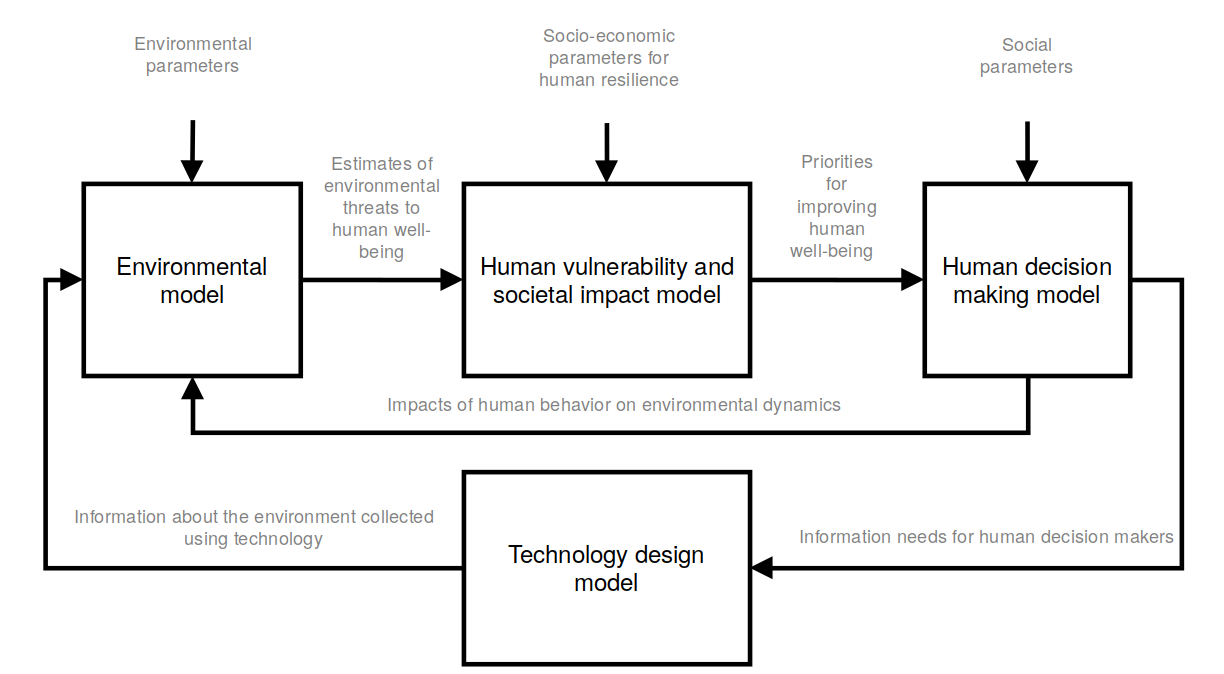
\includegraphics[scale=0.3]{/home/jackreid/Documents/School/Research/Space_Enabled/Thesis/Figures/modelflow.png}
    \caption{ Baseline version of the Environment - Vulnerability - Decision - Technology Model (Generic Case)}
    \label{fig:model}
\end{figure}

This set of four models with the particular linkages shown in Figure \ref{fig:model} are not the only form that \ac{evdt} can take, merely the most general arrangement. Some applications may involve replacing a model with a human-in-the-loop (e.g. having the user themself substitute for the decision-making model) or omitting a model altogether. For other applications, it may make sense to conceptually break a model into two or more components. In the Vida project, it was considered worthwhile to separate the social impact model into two components, one focusing on public health (the obvious priority when dealing with COVID-19) and one focusing on non-health metrics (such as income, employment, etc.). Such a separation can be useful if either significantly different modeling methodologies are going to be used or if the linkages with the other \ac{evdt} components are different from one another. 

One way to determine the optimal arrangment of \ac{evdt} components is to consider what questions the user or researcher is seeking to answer with this application of \ac{evdt}. For instance, the default \ac{evdt} arrangement shown in Figure \ref{fig:model} was motivated primarily by the following four questions:

\begin{enumerate} \setlength{\itemsep}{0pt} \setlength{\parskip}{0pt}
    \item What is happening in the natural environment?
    \item How will humans be impacted by what is happening in the natural environment?
    \item What decisions are humans making in response to environmental factors and why?
    \item What technology system can be designed to provide high quality information that supports human decision making?
\end{enumerate}

Alternate questions may result in a different configuration or set of components. The point of \ac{evdt} is not to insist upon a particular set of linkages and feedbacks, but rather to encourage a consideration of such linkages between domains in general, and to consider them through a systems engineering perspective. Of course answering the structuring questions, and even phrasing them in the first place, requires the use of collaborations. 

\subsection{Case Studies / Study Areas}

While \ac{evdt} does not include any concrete spatial scale requirements, it is often the most straightforward to apply to it at a a relatively local scale, like much of the early history of \ac{gis} applications \cite{tullochInstitutionalGeographicInformation2007}. Most of the applications to date have been at the area of a metropolitan area or that of a small province. The most promising applications tend to be at intersections of rural and urban areas. Urban areas often depend on an area significantly larger than the built-up area for basic resources and ecosystem services, particularly for water, bulky materials, and waste disposal. I will not attempt to strictly define rural and urban here, as the "distinctions are often arbitrary" \cite{tacoliRuralurbanInteractionsGuide1998}. Instead this work will rely upon local definitions of urban, rural, and peri-urban, similarly to the \ac{un} \cite{sachsAgeSustainableDevelopment2015}. 

\subsubsection{Rio de Janeiro Mangroves and Fishing Communitites}

Guaratiba is a relatively rural district of Rio de Janeiro situated in the southwestern corner of the municipality. It is home to a mix of land uses, including decorative plant farming, multiple fishing communities, a military base and training center, a state-run biological reserve, some informal settlements, and a growing ecotourism industry. The biological reserve exists to protect the largest remaining mangrove forest within the municipality. These mangroves are vulnerable due to landward urbanization, including a recently opened urban transit line, and rising sea levels \cite{goldbergEcoMapDecisionsupportTool2018} They provide a variety of ecosystem services, including serving as a mechanism for highly efficient carbon sequestration, supporting a small-scale industry of fishing and crab catching, preventing coastal erosion, and attracting the aforementioned local ecotourism industry \cite{schwenkResearchEnvironmentalSocioeconomical2008}. Government policies to conserve the mangroves can use integrated modeling tools to consider both the benefits of protecting the forests as well as the economic needs of low-income communities. This, coupled with the Rio de Janeiro municipal government's pre-existing interest in generating useful datasets and making them available online through the Data.Rio platform \cite{matheusOpenGovernmentData2014}, made the Guaratiba mangroves a particularly suitable case study for the \ac{evdt} Modeling Framework. Our primary collaborators and points of contact are \ac{ipp}, which is the municipal data agency, and ESPAÇO, a research group at the \ac{ufrj} who study various coastal ecosystems in Brazil and elsewhere \cite{cruzClassificacaoOrientadaObjetos2007, seabraMapeamentoDinamicaCobertura2013} and who are also familiar with examining socioeconomic impacts of environmental phenomena \cite{schwenkResearchEnvironmentalSocioeconomical2008}. This project began in 2018 and since that time Jack Reid made two multi-week field visits to Rio de Janeiro and Guaratiba in particular.


\subsubsection{The Vida COVID-19 Response Project}

As the coronavirus pandemic swept the globe, many of the local points of contact working with Space Enabled on \ac{evdt} and other projects had sudden changes in priorities. Several of them raised the possibility of adapting and expanding the \ac{evdt} Modeling Framework to approach coronavirus-related decision-making and impact analysis. This seemed relevant because, as others have noted, coronavirus impacts and response can be characterized as a complex system warranting a multi-domain, model-based approach \cite{deweckHandlingCOVID192020}. The second case study will focus on this project, which ultimately became known as Vida and came to involve six metropolitan areas across Angola, Brazil, Chile, Indonesia, Mexico, and the United States. In each of these areas, Vida was (and is) developed in collaboration with local government officials, university researchers, and general community members. 

Whereas the first case study focuses on simulating the changes in mangrove forest over decades, the focus of Vida is examining hourly to weekly air and water quality data alongside daily coronavirus epidemiological data and weekly quarantine policies. Government officials need actionable data to both address the ongoing public health crisis and to cope with the resultant socioeconomic and environmental consequences. Community members need to understand why their government is making the decisions that it is and understand the risks associated with their own actions.

\subsection{Development and Evaluation}

%This includes using stakeholder mapping and network analysis to inform the design of the \ac{dss} in question. Other components of the methodology taken in this work are developing the \ac{dss} through an iterative and collaborative process with specific stakeholders; pursuing targeted, related analyses, such as on the value of certain ecosystem services, the value of remote sensing information, and human responses to various policies; and evaluating the usefulness of both the \ac{dss} and the development process through interviews, workshops, and other feedback mechanisms.

It should be acknolwedged that these projects are actively underway, so some parts of the development process described here have already been completed, either partially or in full.

Each of the case studies begins with discussions with potential collaborators who are local to study area. These conversations serve to outline the general scope of the study area and identify other stakeholders. This transitions smoothly into more formal qualitative interviews with representatives of the various stakeholder communities to elicit needs, relationships with other stakeholders, and general perspectives. These are used to construct stakeholder maps which can then be analyzed to identify the \ac{dss} goals and requirements, as well as the context constraints that it will be operating in \cite{crawleySystemArchitectureStrategy2015, woodBuildingTechnologicalCapability2012}. We also seek to understand the history of the area both environmentally and socially, in order to understand the existing systems that we are intervening in, rather than assuming that each location is a sustainable development tabula rasa. The Space Enabled philosophy of research (and thus of \ac{evdt}) involves a level of participation and collaboration that goes beyond stakeholder analysis. By paring complex \ac{sets} theory with such collaborative planning theory, we can thereby avoid many of the traditional problems of systems engineering \cite{goodspeedScenarioPlanningCities2020}. Once initial versions of these are completed, work begins on the actual \ac{dss}. During this process, ongoing meetings with a diverse set of stakeholders continue in order to receive feedback on prototypes, elicit new useful datasets, identify additional needs, and encourage direct contribution to the \ac{dss} code (when desired by the local collaborators). In this way, a certain level of evaluation takes place throughout the development process. Nonetheless, additional validation is required.

For each component of \ac{evdt}, internal validation work is best conducted according to the norms and standards of that field. For the Environment Model in the mangrove case, for example, this entails working with ESPAÇO using both remote sensing and in-situ monitoring in order to calibrate and confirm the results of the mangrove health tracking discussed earlier. In addition to this component-by-component verification work, however, there is also a need for overarching validation of the \ac{evdt} Modeling Framework and its specific instantiation in a particular context. Through the stakeholder analysis process described above, target audiences can be identified and then engaged either individually or as cross-audience groups in directed workshops to assess validity via the collection of methods known as purposeful gaming \cite{rossGamebasedLearningSystems2014}, wargaming \cite{hansonImprovingOperationalWargaming2016,selvaRevitalizingWargamingNecessary15,shlapakReinforcingDeterrenceNATO2016}, and role playing gaming \cite{groganStrategicEngineeringGaming2012,groganFederatedSimulationGaming2012}. One key aspect to note about scope and intent here, is that this work aims to present modeling methods that may support local policymaking, but not generate specific policy recommendations as an outside export, nor to deliver fully operational versions of the \acp{dss} to each case study. 

\section{Expected Results and Contributions}

Each stage of the research plan will result in specific, concrete products.

\textbf{First, the stakeholder interview and need identification process} will result in stakeholder maps (an simplified example of which is shown in Figure \ref{fig:rio_stakemap}) and associated analyses. These in turn will directly inform the systems architecture, a high-level example of which can be seen in Figure \ref{fig:architecture}. Both of these are continuously refined during the collaboration process.

\begin{figure}[h]
	\centering
	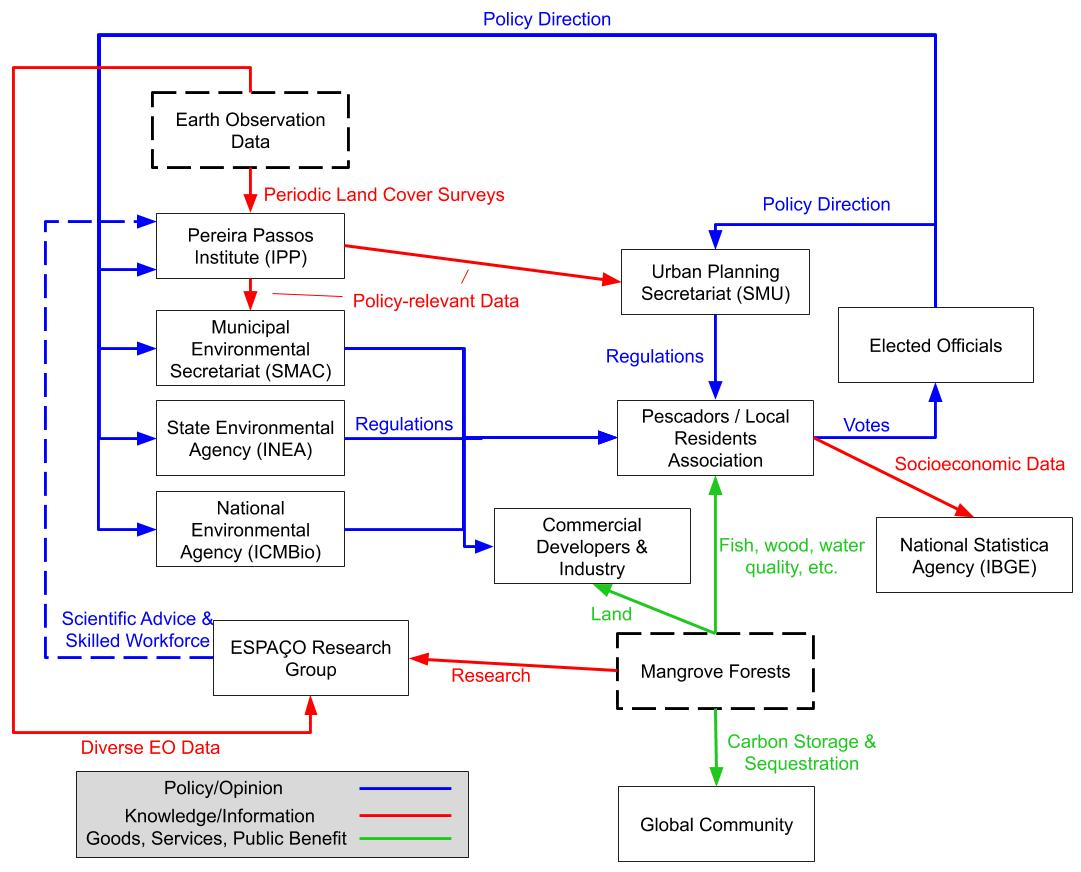
\includegraphics[scale=0.25]{/home/jackreid/Documents/School/Research/Space_Enabled/Thesis/Figures/chap4/Stakeholder_Map_v2.jpg}
	\caption[Stakeholder Map for the Mangrove Forests of Reio de Janeiro]{Stakeholder Map for the Mangrove Forests of Reio de Janeiro}
	\label{fig:rio_stakemap}
\end{figure}

\begin{figure}[h]
	\centering
	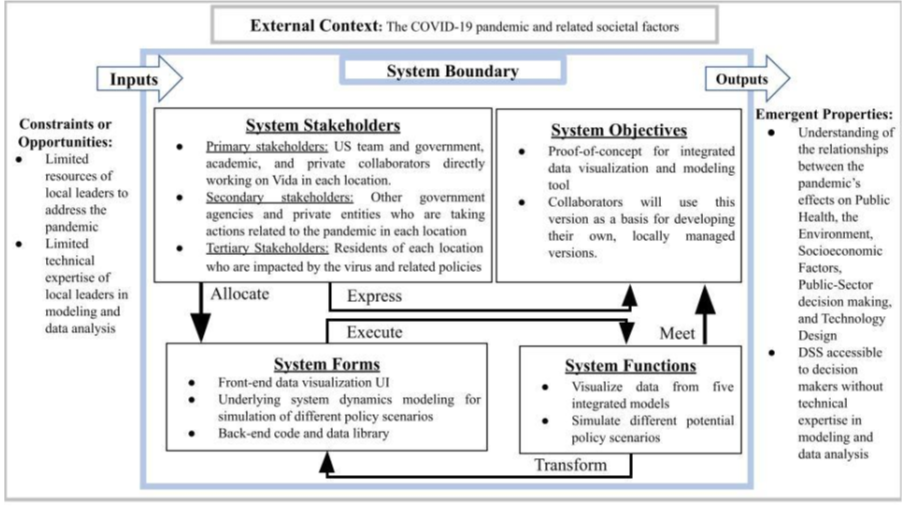
\includegraphics[scale=0.3]{/home/jackreid/Documents/School/Research/Space_Enabled/Thesis/Figures/architecture.png
}
	\caption{The high-level functional systems architecture of the Vida \ac{dss}.}
	\label{fig:architecture}
\end{figure}


\textbf{Second, the \ac{dss} development process} will result in both intermediary and final products. The intermediary products include \ac{evdt}-component analyses, such as assessments of mangrove health and extent over time, and the identification of inter-component linkages, such as quantifications of mangrove ecosystem services or the quantification of the impacts of COVID-19 on human activity as measured by urban nightlights and telecoms mobility data. Final products include the prototype \ac{dss} software themselves which can continue to be used and developed following the conclusion of this work.

\textbf{Third, the evaluation process} will result in the identification of (a) whether \ac{evdt} \acp{dss} have the potential to improve the management of earth observation and socioeconomic data in a format usable by non-exper and (b) how to improve and expand the \ac{evdt} framework moving forward. In the long run, \ac{evdt} is not intended to be an exclusive project of Space Enabled. Once \ac{evdt} has been refined and demonstrated through this and other projects, the next step will be to consolidate and standardize the underlying code, so as to facilitate furture improvements, as well as the reuse of materials for future contexts. The open source code repositories, already available online \cite{bluerasterBlueRasterVida2021,reidEVDTRepository2020,reidMITVidaRepository2021}, will be used as a basis for building a community of practice, where individuals can contribute in a variety of ways, as shown in Figure \ref{fig:development}. As the number of applications increase and the code is refined, the various models used in the applications may themselves be the first members of an openly accessible library of models. Potential user groups could adapt and reuse \ac{evdt} components in other applications, without having to start from scratch. Initially this would likely still require significant code expertise, but it is entirely possible for functionality to be created to allow for `plug-and-play.' A user may be able to, in browser or on desktop, select a geographic area of interest (e.g. the Sóc Trăng Province of Vietnam), select an environmental model (e.g. coastal forest health), a societal impact model (e.g. cyclone vulnerability), a decision-making model (land use conversion and conservation policy), and a technology model (satellite versus in-situ monitoring), all without writing a line of code (though perhaps being required to import new datasets themselves).

\begin{figure}[h]
	\centering
	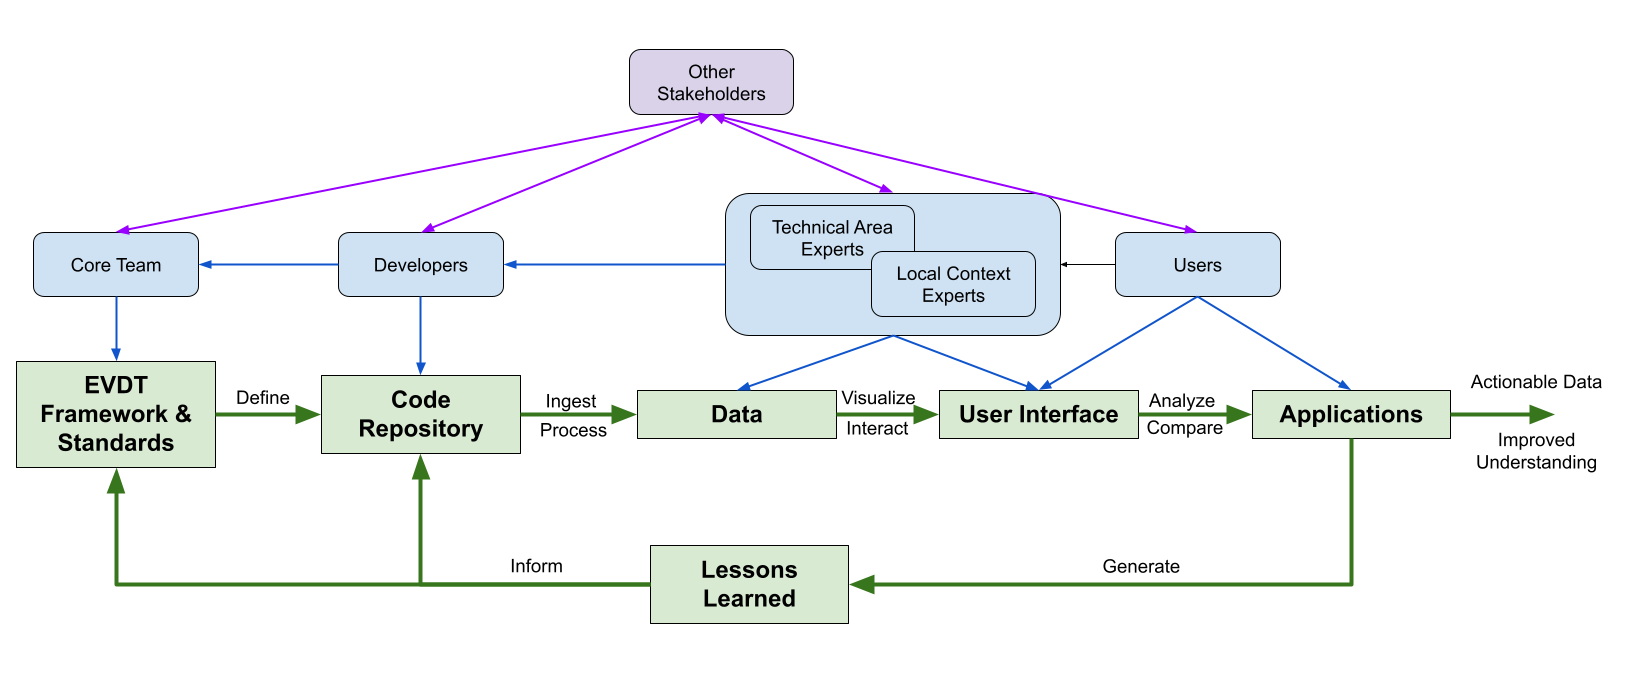
\includegraphics[scale=0.25]{/home/jackreid/Documents/School/Research/Space_Enabled/Thesis/Figures/Graphic_2_Development.png}
	\caption{The EVDT development pipeline. Note that the different community groups, shown in blue, are not necessarily discrete and one individual could simultaneously participate in multiple.}
	\label{fig:development}
\end{figure}

\textbf{Fourth, the overall process} will advance the contribute to a variety of broader societal impacts. These include:
\begin{itemize}
	\item Encourage the joint consideration of both human and environmental systems in a dynamic, continual fashion, thereby avoiding some of the negative consequences of siloed, static conservation mapping practices \cite{harrisRethinkingMapsMorethanhuman2011}. 
	\item Expand the population of \ac{eo} data users by increasing accessibility and demonstrating utility of \ac{eo} data to policymaking.
	\item Reduce burden of facilitation by space agencies. Many national space agencies are focused primarily on scientific missions. While they are often happy to assist other groups in using the data that their satellites generate, they often have limited resources and time to do so. For instance, the famous \textit{Pale Blue Dot} photograph from taken by Voyager 1 after the conclusion of its primary mission, almost did not happen, as the photo had no scientific value and arranging for the shot required money and experts who had already been reassigned to other missions \cite{greenfieldboycePaleBlueDot2010}. Integrated models could potentially enable the application organizations to be less reliant on direct assistance from space agencies, thereby freeing up space agency resources for other applications.
\end{itemize}

\newpage

\bibliography{/home/jackreid/Documents/School/Research/Space_Enabled/Thesis/main}
\bibliographystyle{unsrt}

\end{document}
